\documentclass[
	12pt,				% tamanho da fonte
	openany,			% capítulos começam em pág ímpar (insere página vazia caso preciso)
	oneside, 			% oneside - twoside
	a4paper,			% tamanho do papel.
	chapter=TITLE,		% títulos de capítulos convertidos em letras maiúsculas
	section=TITLE,		% títulos de seções convertidos em letras maiúsculas
	sumario=tradicional,
	%subsection=TITLE,	% títulos de subseções convertidos em letras maiúsculas
	%subsubsection=TITLE,% títulos de subsubseções convertidos em letras maiúsculas
	english,			% idioma adicional para hifenização
	brazil,				% o último idioma é o principal do documento
	]{abntex2}

% ---------------------------------------------------------------------------
% Inclui os comandos do projeto
% ---------------------------------------------------------------------------
% -----------------------------------------------------------------------------
% Pacotes fundamentais
% -----------------------------------------------------------------------------
\usepackage{xcolor}
\newcommand\myworries[1]{\textcolor{red}{[#1]}}
\usepackage{lmodern}		% Usa a fonte Latin Modern (Serifada, tipo Times New Roman
%\usepackage{helvet}		% Usa a fonte Helvetica (Tipo Arial)
%\renewcommand{\familydefault}{\sfdefault} tira o serifado
\usepackage[T1]{fontenc}		% Selecao de codigos de fonte.
\usepackage[utf8]{inputenc}		% Codificacao do documento (conversão automática dos acentos)
\usepackage{indentfirst}		% Indenta o primeiro parágrafo de cada seção.
\usepackage{color}				% Controle das cores
\usepackage{tikz}				% Inclusão de gráficos
\usepackage{graphicx}			% Inclusão de gráficos
\usepackage{microtype} 			% para melhorias de justificação
% -----------------------------------------------------------------------------
% Pacotes adicionais, usados no anexo do modelo de folha de identificação
% -----------------------------------------------------------------------------
\usepackage{multicol}
\usepackage{multirow}
% -----------------------------------------------------------------------------
% Pacotes adicionais, usados apenas no âmbito do Modelo Canônico do abnteX2
% -----------------------------------------------------------------------------
\usepackage{lipsum}				% para geração de dummy text
% -----------------------------------------------------------------------------
% Pacotes de citações
% -----------------------------------------------------------------------------
\usepackage[brazilian,hyperpageref]{backref}	 % Paginas com as citações na bibliografia
\usepackage[alf,abnt-etal-list=3,abnt-etal-cite=2, abnt-emphasize=bf,abnt-repeated-author-omit=yes,abnt-etal-text=emph]{abntex2cite}	% Citações padrão ABNT
\usepackage{pdflscape}
\usepackage{footnote}
\usepackage{pdfpages}
\usepackage{caption}

% -----------------------------------------------------------------------------
% Pacotes adicionados por @leolleocomp
% -----------------------------------------------------------------------------
\usepackage{booktabs}
\usepackage{adjustbox}
\usepackage{subcaption}
\usepackage[labelfont=bf]{caption}
\usepackage{gensymb}
\usepackage{amsmath}
\usepackage{array}
% \usepackage{float}
\usepackage{xcolor,colortbl}
\usepackage{longtable}
\usepackage{scalefnt}
\usepackage{listings}			% inserir codigo fonte
\usepackage{morewrites} % necessário pois estamos screvendo muitos arquivos
\usepackage{enumitem}

% -----------------------------------------------------------------------------
% Pacotes adicionados por @Gabrielr2508
% -----------------------------------------------------------------------------
\usepackage{hyperref}

\usepackage{tocloft}
% -- permite a adição de células especiais em tabelas
\newcommand{\specialcell}[2][c]{%
  \begin{tabular}[#1]{@{}c@{}}#2\end{tabular}}

\newcounter{equationset}
\newcommand{\equationset}[1]{% \equationset{<caption>}
  \refstepcounter{equationset}% Step counter
  \noindent\makebox[\linewidth]{Equação ~\theequationset: #1}
 }

%-------------------------------------------------------------------------------
% Adequação dos títulos dos capitulos, seções, subseções às normas da Univasf
% Added by @Gabrielr2508
%-------------------------------------------------------------------------------
\renewcommand{\ABNTEXchapterfont}{\fontseries{b}}
\renewcommand{\ABNTEXchapterfontsize}{\normalsize}

\renewcommand{\ABNTEXsectionfont}{\fontseries{m}}
\renewcommand{\ABNTEXsectionfontsize}{\normalsize}

\renewcommand{\ABNTEXsubsectionfont}{\fontseries{b}}
\renewcommand{\ABNTEXsubsectionfontsize}{\normalsize}

\renewcommand{\ABNTEXsubsubsectionfont}{\fontseries{m}}
\renewcommand{\ABNTEXsubsubsectionfontsize}{\normalsize}

%-------------------------------------------------------------------------------
% CONFIGURAÇÕES DE PACOTES
% Configurações do pacote backref
%-------------------------------------------------------------------------------
% Usado sem a opção hyperpageref de backref
\renewcommand{\backrefpagesname}{Citado na(s) página(s):~}
% Texto padrão antes do número das páginas
\renewcommand{\backref}{}
% Define os textos da citação
\renewcommand*{\backrefalt}[4]{
  \ifcase #1 %
    %Nenhuma citação no texto.%
  \or
    Citado na página #2.%
  \else
    Citado #1 vezes nas páginas #2.%
  \fi}%

%-------------------------------------------------------------------------------
% Configurações de aparência do PDF final
%-------------------------------------------------------------------------------
% alterando o aspecto da cor azul
\definecolor{blue}{RGB}{41,5,195}

% informações do PDF
\makeatletter
\hypersetup{
       %pagebackref=true,
    pdftitle={\@title},
    pdfauthor={\@author},
      pdfsubject={\imprimirpreambulo},
      pdfcreator={LaTeX with abnTeX2},
    pdfkeywords={abnt}{latex}{abntex}{abntex2}{relatório técnico},
    colorlinks=true,			% false: boxed links; true: colored links
      linkcolor=black,				% color of internal links
      citecolor=black,				% color of links to bibliography
      filecolor=black,			% color of file links
    urlcolor=black,
    bookmarksdepth=4
}
\makeatother
% ---

% ---
% Espaçamentos entre linhas e parágrafos
% ---

% O tamanho do parágrafo é dado por:
\setlength{\parindent}{1.3cm}

% Controle do espaçamento entre um parágrafo e outro:
\setlength{\parskip}{0.2cm}  % tente também \onelineskip

%-------------------------------------------------------------------------------
% compila o indice
%-------------------------------------------------------------------------------
\makeindex
% ---

%-------------------------------------------------------------------------------
% Comando para inserir imagens de forma simples
%-------------------------------------------------------------------------------
\newcommand{\imagem}[4]
{% \imagem{x.x}{nomeimg}{titulo}{fonte}
  \begin{figure}[!htb]
    \caption{\label{img:#2}#3}
    \begin{center}
      \includegraphics[scale=#1]{img/#2}
    \end{center}
        \legend{\textbf{Fonte:} #4.}
  \end{figure}
}%

%-------------------------------------------------------------------------------
% Creio que esses comandos sejam para desenhar algo, aguardando explicações de @leolleocomp
%-------------------------------------------------------------------------------
\newcommand{\xx} {$\bigotimes$}
\newcommand{\oo} {$\bigcirc$}

%-------------------------------------------------------------------------------
% Biblioteca para códigos-fonte
%-------------------------------------------------------------------------------
\usepackage[newfloat=true]{minted}
\usemintedstyle{bw} % Coódigos em preto branco

%-------------------------------------------------------------------------------
% Caixas batutas - by @leolleocomp
%-------------------------------------------------------------------------------
\usepackage[most]{tcolorbox}
\tcbuselibrary{breakable}

\tcbuselibrary{minted}
\tcbset{listing engine=minted}

\definecolor{bg}{rgb}{0.95,0.95,0.95}

\SetupFloatingEnvironment{listing}{name=Código, listname=Lista de códigos}

%-------------------------------------------------------------------------------
% configuração do contador dos códigos-fonte - by @leolleocomp
% assim como as figuras, começa em 1
\newcounter{sourcecode}
%-------------------------------------------------------------------------------
%-------------------------------------------------------------------------------
% @leolleocomp
% stackoverflow code
% peguei da resposta abaixo
% https://stackoverflow.com/questions/24086366/change-latex-minted-listings-numbering-to-include-current-section?answertab=votes#tab-top
%-------------------------------------------------------------------------------
\makeatletter
\renewcommand*{\thelisting}{\thesourcecode}
\makeatother

%-------------------------------------------------------------------------------
% Peçam explicações a @leolleo
% WHO DID THIS?
%-------------------------------------------------------------------------------
\newcommand{\Ididthis}{
%	\legend{\textbf{Fonte:} O autor (\the\year).}
\legend{\textbf{Fonte:} Elaborado pelo autor.}
}

\newcommand{\Otherguydidthis}[1]{
  \legend{\textbf{Fonte:} \citeonline{#1}.}
}

%-------------------------------------------------------------------------------
% Comando para inserir códigos - by @leolleocomp
%-------------------------------------------------------------------------------
\newcommand{\sourcecode}[4]{
\begin{listing}[h]
  \refstepcounter{sourcecode}
  \caption{#1}
  \label{cmd:#2}
  \inputminted[linenos, bgcolor=bg, tabsize=2,breaklines,fontsize=\scriptsize]{#3}{codes/#4}
  \Ididthis
\end{listing}
}


% -----------------------------------------------------------------------------
% Pacotes adicionados por @ruanmed
% -----------------------------------------------------------------------------
\usepackage[binary-units=true]{siunitx}


%-------------------------------------------------------------------------------
% Comando para inserir códigos - by @ruanmed
%-------------------------------------------------------------------------------
\usepackage{caption}

\newenvironment{code}{\captionsetup{type=listing}}{}
\SetupFloatingEnvironment{listing}{name=Código}

\newcommand{\sourcecodenolist}[3]{
  \begin{code}
      \refstepcounter{sourcecode}
        \captionof{listing}{#1 }
        \inputminted[bgcolor=bg, tabsize=2,breaklines,fontsize=\scriptsize, bgcolor=white]{#2}{codes/#3}
        \Ididthis
    \end{code}
}

\newcommand{\sourcecodeinline}[2]{
  \mintinline[linenos, bgcolor=bg, tabsize=4,breaklines]{#1}{#2}
}


% CONFIGURACAO DO SUMARIO
%-------------------------------------------------------------------------------
% Modifica o espaçamento no sumário
% Nao ha espacos, exceto para as entradas de capitulos
\setlength{\cftbeforeparagraphskip}{0pt}
\setlength{\cftbeforesubsectionskip}{0pt}
\setlength{\cftbeforesectionskip}{0pt}
\setlength{\cftbeforesubsubsectionskip}{0pt}
\setlength{\cftbeforechapterskip}{\onelineskip}

% Alteração da indentação dos itens do sumário
\cftsetindents{chapter}{0pt}{42pt}
\cftsetindents{section}{0pt}{42pt}
\cftsetindents{subsection}{0pt}{42pt}
\cftsetindents{subsubsection}{0pt}{42pt}

% Modifica a formatacao dos textos

% Secao Primaria (Chapter): Caixa alta, Negrito, tamanho 12
\makeatletter
\settocpreprocessor{chapter}{%
  \let\tempf@rtoc\f@rtoc%
  \def\f@rtoc{%
  \texorpdfstring{\bfseries\MakeTextUppercase{\tempf@rtoc}}{\tempf@rtoc}}%
}
\makeatother

% Novo list of (listings) para QUADROS
% retirado de https://github.com/abntex/abntex2/wiki/HowToCriarNovoAmbienteListing

\newcommand{\quadroname}{Quadro}
\newcommand{\listofquadrosname}{Lista de quadros}

\newfloat[chapter]{quadro}{loq}{\quadroname}
\newlistof{listofquadros}{loq}{\listofquadrosname}
\newlistentry{quadro}{loq}{0}

% configurações para atender às regras da ABNT
\setfloatadjustment{quadro}{\centering}
\counterwithout{quadro}{chapter}
\renewcommand{\cftquadroname}{\quadroname\space}
\renewcommand*{\cftquadroaftersnum}{\hfill--\hfill}

% Configuração de posicionamento padrão:
\setfloatlocations{quadro}{hbtp}

% Trocar o título da lista de ilustrações para lista de figuras
\addto\captionsbrazil{
  \renewcommand{\listfigurename}
    {Lista de figuras}
}


% ---------------------------------------------------------------------------
% IDENTIFICAÇÃO
% ---------------------------------------------------------------------------
\titulo{AVALIAÇÃO DE MODELOS PREDITIVOS DE EVASÃO NA EAD, BASEADOS NA TEORIA DA DISTANCIA TRANSACIONAL}
\autor{ESRON DTAMAR DA SILVA}
\local{JUAZEIRO - BA}
\orientador{Prof. Dr. Jorge Luis Cavalcanti Ramos}
%\coorientador{M. Sc. Osvaldo Campelo de Mello Vasconselos}
\instituicao{
UNIVERSIDADE FEDERAL DO VALE DO SÃO FRANCISCO
	\par
CURSO DE GRADUAÇÃO EM ENGENHARIA DE COMPUTAÇÃO}
\tipotrabalho{Trabalho de Conclusão de Curso}
\preambulo{Trabalho apresentado à Universidade Federal do Vale do São Francisco - Univasf, \textit{Campus} Juazeiro, como requisito da obtenção do título de Bacharel em Engenharia de Computação.}


% -----------------------------------------------------------------------------
% CONFIGURACAO DO SUMARIO - by @Gabrielr2508
% Precisa estar aqui, por isso não foi para o commands.tex, não descobrimos o motivo, %caso saiba, por favor, faça um pull request! :D
% -----------------------------------------------------------------------------
% Secao primaria (Chapter) Caixa alta, Negrito, tamanho 12
\makeatletter
\renewcommand*{\l@chapter}[2]{%
  \l@chapapp{\uppercase{#1}}{#2}{\cftchaptername}}
\makeatother
% Secao secundaria (Section) Caixa baixa, Negrito, tamanho 12
\renewcommand{\cftsectionfont}{\uppercase} %ponha \rmfamily se quiser serifadas...

% Secao terciaria (Subsection) Caixa baixa, negrito, tamanho 12
\renewcommand{\cftsubsectionfont}{\bfseries}

% Secao quaternaria (Subsubsection) Caixa baixa, tamanho 12
\renewcommand{\cftsubsubsectionfont}{\normalfont}

% Seção quinaria (subsubsubsection) Caixa baixa, sem negrito, tamanho 12
\renewcommand{\cftparagraphfont}{\normalfont\itshape}

% -----------------------------------------------------------------------------
% Início do TCC
% -----------------------------------------------------------------------------
\begin{document}

	\frenchspacing % Retira espaço extra obsoleto entre as frases.

	\pretextual
		%-------------------------------------------------------------------------------
% Constrói a capa com base na seção de identificação do main.tex
%-------------------------------------------------------------------------------
\begin{capa}
    \setlength{\belowcaptionskip}{0pt}
    \setlength{\abovecaptionskip}{0pt}
    \setlength{\intextsep}{-18pt}
        \begin{figure}[h]
        \begin{center}
            \includegraphics[scale=1.0]{img/LOGO_UNIVASF_big.pdf}
        \end{center}
      \end{figure}

        %\includegraphics[scale=0.6]{img/univasf.jpg}
        \center
      {\ABNTEXchapterfont\large\imprimirinstituicao}

      \vspace*{2cm}
          {\imprimirautor}
      \vspace*{2cm}
        \begin{center}
        \ABNTEXchapterfont\bfseries\large\imprimirtitulo
        \end{center}
      \vfill

      \ABNTEXchapterfont\bfseries\large\imprimirlocal\\
      \the\year

      \vspace*{1cm}
\end{capa}
%-------------------------------------------------------------------------------
% Constrói a folha de rosto com base na seção de identificação do main.tex
%-------------------------------------------------------------------------------
\begin{folhaderosto}
    \center
      {\ABNTEXchapterfont\large\imprimirinstituicao}

    \vspace*{2cm}
          {\imprimirautor}
      \vspace*{2cm}
    \vspace*{\fill}

    {\ABNTEXchapterfont\bfseries\large\imprimirtitulo}
    \vspace*{\fill}

    {\hspace{.45\textwidth}
    \begin{minipage}{.5\textwidth}
      \SingleSpacing
      \imprimirpreambulo \\ \\

      {\imprimirorientadorRotulo~\imprimirorientador\par}
      {\imprimircoorientadorRotulo~\imprimircoorientador\par}

    \end{minipage}%
    \vspace*{\fill}}%
    \vspace*{\fill}
      \ABNTEXchapterfont\bfseries\large\imprimirlocal\\
      \the\year
    \vspace*{1cm}
\end{folhaderosto}

%-------------------------------------------------------------------------------
% Constrói a ficha catalográfia com base na seção de identificação do main.tex
% Está comentado porque no final das contas a biblioteca do seu campus que gera a
% numeração, você pode adicionar os numeros aqui, ou anexar o pdf gerado por eles
% ao documento.
%-------------------------------------------------------------------------------
%\begin{fichacatalografica}
%	\vspace*{\fill}					% Posição vertical
%	\hrule							% Linha horizontal
%	\begin{center}					% Minipage Centralizado
%	\begin{minipage}[c]{12.5cm}		% Largura
%
%	\imprimirautor
%
%	\hspace{0.5cm} \imprimirtitulo  / \imprimirautor. --
%	\imprimirlocal, \the\year-
%
%	\hspace{0.5cm} xx p. : il. (algumas color.) ; 30 cm.\\
%
%	\hspace{0.5cm} \imprimirorientadorRotulo~\imprimirorientador\\
%
%	\hspace{0.5cm}
%	\parbox[t]{\textwidth}{\imprimirtipotrabalho~--~\imprimirinstituicao,
%	\the\year.}\\
%
%	\hspace{0.5cm}
%		1. Palavra-chave1.
%		2. Palavra-chave2.
%		I. Orientador.
%		II. Universidade xxx.
%		III. Faculdade de xxx.
%		IV. Título\\
%
%	\hspace{8.75cm} CDU 02:141:005.7\\
%
%	\end{minipage}
%	\end{center}
%	\hrule
%\end{fichacatalografica}

%--------------------------------------------------------------------------------
% Anexando a ficha catalogáfica e a folha de aprovação
%--------------------------------------------------------------------------------
% 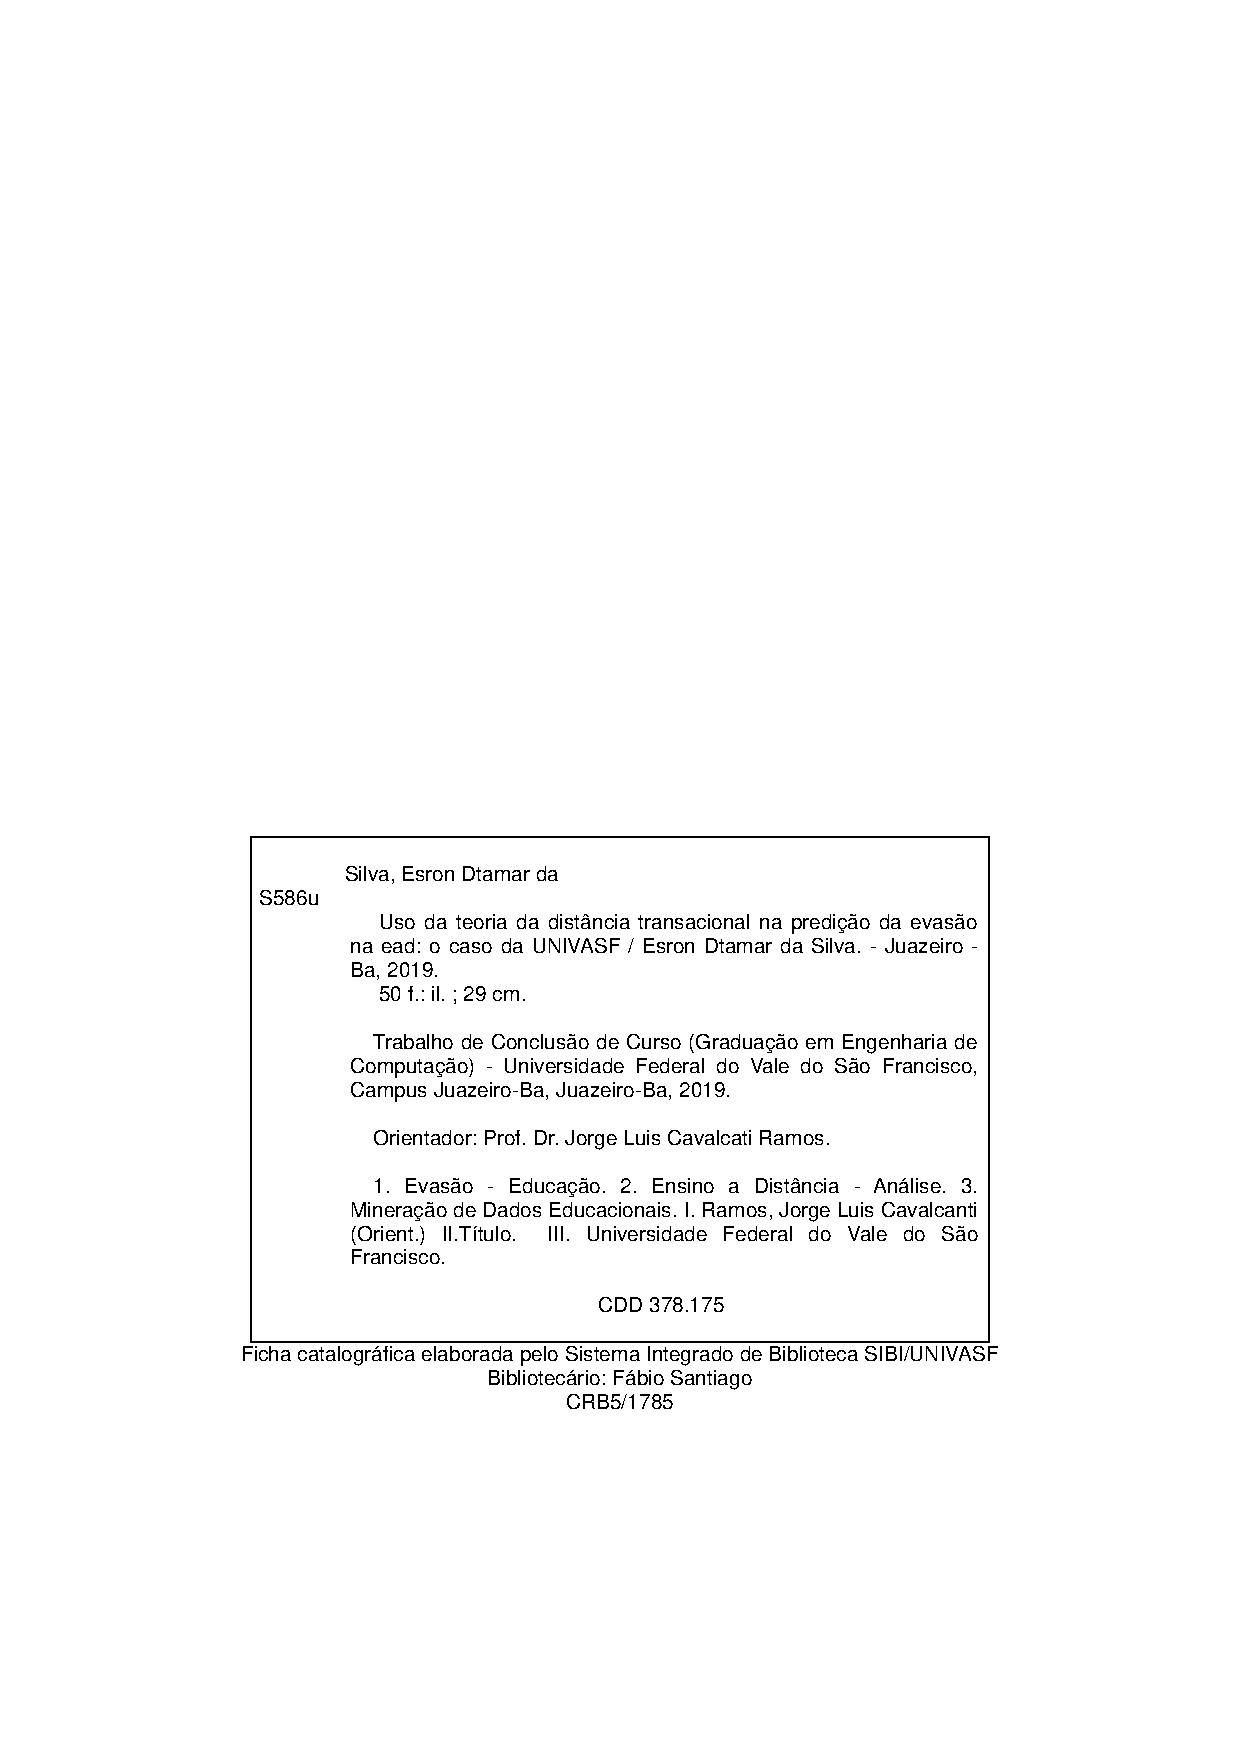
\includepdf[pages=-]{anexos/ficha.pdf}

% 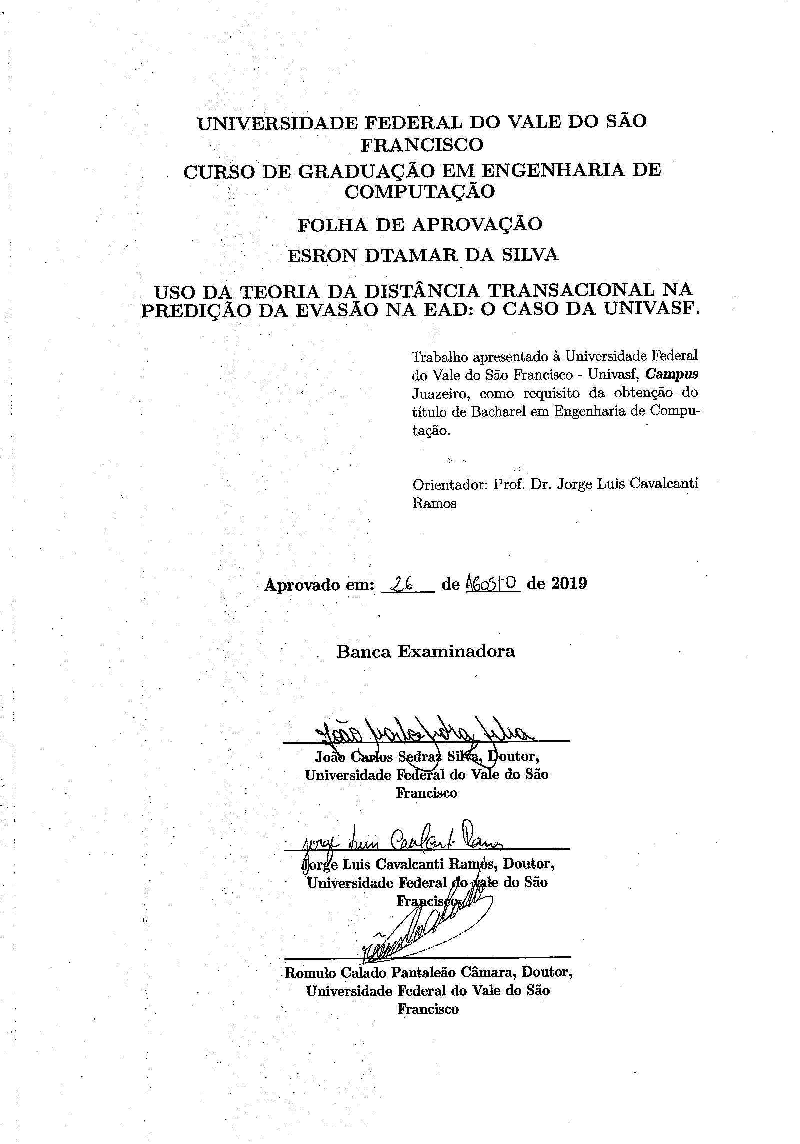
\includepdf[pages=-]{anexos/aprovacao.pdf}

% \setlength{\ABNTEXsignwidth}{12cm}

%--------------------------------------------------------------------------------
% Está comentado pelo mesmo motivo da ficha catalográfica
%--------------------------------------------------------------------------------
%\begin{folhadeaprovacao}
%	\begin{center}
%	    {\ABNTEXchapterfont\bfseries\large\imprimirinstituicao}
%	    \vspace*{\fill}
%
%	    {\ABNTEXchapterfont\bfseries\large FOLHA DE APROVAÇÃO}
%	    \vspace*{\fill}
%
%	    {\ABNTEXchapterfont\bfseries\large\imprimirautor}
%
%	    \vspace*{\fill}\vspace*{\fill}
%	    {\ABNTEXchapterfont\bfseries\large\imprimirtitulo}
%	    \vspace*{\fill}
%
%	    {\hspace{.45\textwidth}
%		\begin{minipage}{.5\textwidth}
%			\SingleSpacing
%			\ABNTEXchapterfont\imprimirpreambulo \\ \\
%
%			{\ABNTEXchapterfont\imprimirorientadorRotulo~\imprimirorientador\par}
%			{\ABNTEXchapterfont\imprimircoorientadorRotulo~\imprimircoorientador\par}
%
%		\end{minipage}%
%	    \vspace*{\fill}}
%	\end{center}
%
%	\vspace*{\fill}
%
%	\begin{center}
%			 \ABNTEXchapterfont\large Aprovado em: \_\_\_\_ de \_\_\_\_ de 2017
%	\end{center}

%	\vspace*{\fill}

%	\begin{center}
%			 \ABNTEXchapterfont\bfseries\large Banca Examinadora
%	\end{center}
%
%   \ABNTEXchapterfont\assinatura{Fábio Nelson de Sousa Pereira, Mestre, Universidade Federal do Vale do São Francisco}
%	\ABNTEXchapterfont\assinatura{Jorge Luis Cavalcanti Ramos, Doutor, Universidade Federal do vale do São Francisco}
%  \ABNTEXchapterfont\assinatura{Ricardo Argenton Ramos, Doutor, Universidade Federal do Vale do São Francisco}
%	 \vspace*{\fill}


%\end{folhadeaprovacao}

%-------------------------------------------------------------------------------
% Insere a epígrafe
%-------------------------------------------------------------------------------
% \newpage
% \vspace*{\fill}
% \begin{flushright}
%     \textit{Lorem Ipsum...}
% \end{flushright}

%-------------------------------------------------------------------------------
% Seção de agradecimentos
%-------------------------------------------------------------------------------
% \begin{agradecimentos}

% \lipsum[2-4]

% \end{agradecimentos}

%-------------------------------------------------------------------------------
% Insere a segunda epígrafe
%-------------------------------------------------------------------------------
% \begin{epigrafe}
%   \vspace*{\fill}
%   \begin{flushright}
%     Se pude enxergar a tão grande distância, foi subindo nos ombros de gigantes.\\
%      \vspace{\baselineskip}
%     \textbf{Isaac Newton}\\
%     \textbf{Carta à Robert Hooke, 1676}
%   \end{flushright}
% \end{epigrafe}



%-------------------------------------------------------------------------------
% Seção de resumos
%-------------------------------------------------------------------------------
% resumo em português
\setlength{\absparsep}{18pt} % ajusta o espaçamento dos parágrafos do resumo
\begin{resumo}

  Os avanços do acesso às tecnologias da informação criou um ambiente fértil
  para a pesquisa na área de educação a distância (EAD). Porém, apesar da grande
  disponibilidade e flexibilidade, os cursos da modalidade EAD, no Brasil, ainda
  sofrem com o problema da evasão de estudantes. Acompanhando o crescimento da
  EAD, se desenvolve também a área de Mineração de Dados Educacionais (MDE).
  Este trabalho propõe a utilização de uma metodologia fundamentada em técnicas
  de MDE com o objetivo de construir e avaliar modelos de classificação da
  situação final de estudantes da EAD entre duas classes, evadidos e não
  evadidos usando os algoritmos de aprendizagem de máquina: KNN, Regressão
  Logística e Árvore de Decisisão. Na construção dos modelos, foram utilizados
  dados obtidos de duas turmas no contexto da Universidade Federal do Vale do
  São Francisco (UNIVASF), e, alem disso, as variáveis preditoras foram
  concebidas a partir dos construtos da Teoria da Distância Transacional (TDT).
  Os resultados apontam que essas variáveis podem ser usadas como fontes de
  dados dos classificadores, alcançando valores similares ao estudo original que
  deu origem à este trabalho e em relação aos verificados em trabalhos
  similares.

  \textbf{Palavras-chave}: Educação a distância. Mineração de dados
  educacionais. Evasão. Aprendizagem de máquina

\end{resumo}
\newpage

% resumo em inglês
\begin{resumo}[Abstract]
\begin{otherlanguage*}{english}

  % TODO: refazer a tradução do resumo.
  The advances in information technologies created a very fertile research
  environment in the distance education field. However, despite of the great
  disponibility and flexibility, the   brazilian DE course genre still suffers
  from the students evasion problem, as shown by the EAD.BR census in the last
  few years. Along with the growing in DE, the Educational Data Mining is
  developing as well. Inspired by the Transactional Distance Theory, this works
  proposes the using of knowledge discovery in databases to construct and
  compare classification models on the final situation of a DE student between
  two classes, evasor and not-evasor. This work applies the methodology proposed
  by Ramos et al (2016), adapted to the EAD context in UNIVASF, where the variables utilized in the predictive models
  are constructed based on the TDT attributes, comparing the results found with
  a new educational scenario.

  \textbf{Key-words}: Distance education. Educational data mining. School
  evasion.

\end{otherlanguage*}
\end{resumo}


%-------------------------------------------------------------------------------
% Insere lista de ilustrações
%-------------------------------------------------------------------------------
\begin{KeepFromToc} % Este comando evita que todas as seções dentro dele de apareçam no sumário
\pdfbookmark[0]{\listfigurename}{lof}
\listoffigures
\cleardoublepage


%-------------------------------------------------------------------------------
% Insere lista de tabelas
%-------------------------------------------------------------------------------
\pdfbookmark[0]{\listtablename}{lot}
\listoftables
\cleardoublepage

%-------------------------------------------------------------------------------
% Insere lista de quadros
%-------------------------------------------------------------------------------
\pdfbookmark[0]{\listofquadrosname}{loq}
\listofquadros*
\cleardoublepage

%-------------------------------------------------------------------------------
% Ajusta lista de código - alterar de figures para códigos - by @Gabrielr2508
%-------------------------------------------------------------------------------
% \makeatletter
% \let\l@listing\l@figure
% \def\newfloat@listoflisting@hook{\let\figurename\listingname}
% \makeatother

%-------------------------------------------------------------------------------
% Insere lista de códigos - by @leolleocomp
%-------------------------------------------------------------------------------
% \listoflistings

\end{KeepFromToc}

%-------------------------------------------------------------------------------
% Insere lista de abreviaturas e siglas
%-------------------------------------------------------------------------------
\begin{siglas}
  \item[ABED] Associação Brasileira de Educação a Distância
  \item[AVA] Ambiente Virtual de Aprendizagem
  \item[CFA] Análise Fatorial Confirmatória
  \item[CSV] \textit{Comma Separeted Value}
  \item[DM] \textit{Data Mining}
  \item[DT] Distância Transacional
  \item[EAD] Educação a Distância
  \item[EDM] \textit{Educational Data Mining}
  \item[IDE] \textit{Integrated Development Environment}
  \item[IES] Instituição de ensino superior
  \item[INEP] Instituto Nacional de Estudos e Pesquisas Educacionais Anísio Teixeira
  \item[KDD] \textit{Knowledge Discovery in Databases}
  \item[KNN] \textit{K-nearest Neighbors}
  \item[LA] \textit{Learning Analytics}
  \item[LMS] \textit{Learning Management System}
  \item[ML] \textit{Machine Learning}
  \item[RL] Regressão Logística
  \item[SEAD] Secretaria de Educaçao a Distância
  \item[SGBD] Sistema de Gerenciamento de Banco de Dados
  \item[SQL] \textit{Structured Query Language}
  \item[STI] Secretaria de Tecnologia da Informação
  \item[SVM] \textit{Support Vector Machine}
  \item[TCC II] Trabalho de Conclusão de Curso II
  \item[TDT] Teoria da Distância Transacional
  \item[UNIVASF] Universidade Federal do Vale do São Francisco
\end{siglas}

%-------------------------------------------------------------------------------
% Insere o sumario
%-------------------------------------------------------------------------------
\pdfbookmark[0]{\contentsname}{toc}
\tableofcontents*
\cleardoublepage


	\textual
		\pagestyle{simple}
		%--------------------------------------------------------------------------------------
% Este arquivo contém a sua introdução, objetivos e organização do trabalho
%--------------------------------------------------------------------------------------
\chapter{Introdução}

O desafio de levar educação e formação profissional a lugares remotos, onde,
dificilmente, a formação presencial tradicional conseguiria alcançar de maneira
efetiva, é uma das principais bandeiras da Educação a Distância (EAD).
Entretanto, outros desafios surgem em decorrência da expansão da modalidade:
como garantir a qualidade dessa formação? como transpor modelos de educação
presencial para a distância? como atuar de maneira a prevenir e reduzir os altos
índices de evasão, ainda verificados na modalidade? São questões como essas que
devem ser respondidas a partir do desenvolvimento de pesquisas nessa modalidade.
O uso de novas tecnologias e de novos processos podem contribuir com essas
pesquisas.

Diversas iniciativas reforçam o crescimento da EAD e exigem uma atenção maior
nos aspectos importantes para a consolidação e manutenção das atividades dessa
modalidade nas instituições. Dentre esses aspectos, está a necessidade de
pesquisas, como forma de se agregar procedimentos validados cientificamente,
ferramentas de gestão mais eficientes e metodologias inovadoras, capazes de
superar grandes desafios impostos pela EAD.

O avanço da modalidade de EAD requer o desenvolvimento de recursos que permitam
o acompanhamento de cursos oferecidos em um ambiente virtual de aprendizagem.
Esses recursos podem ser obtidos a partir de metodologias de análise que
envolvem o conhecimento das estratégias pedagógicas dos cursos EAD, o
levantamento das necessidades apontadas pelos profissionais que atuam na área e
na elicitação dos requisitos para implementação de ferramentas de visualização
de dados de diversas atividades dentro de um contexto educacional.
\cite{ramos2016abordagem}

Com a expansão do EAD de maneira responsável e planejada, com infraestrutura
compatível e recursos humanos qualificados, será possível a oferta de novos
cursos pelas instituições, disseminando conhecimento e possibilitando mais
oportunidades para o desenvolvimento regional.

Para \citeonline{ramos2016abordagem}, os altos índices de evasão dos alunos em
cursos EAD representam um grande desafio para todos os que atuam na modalidade.
Além desses índices estarem em níveis elevados, observou-se também que estão em
crescimento. Com isso há uma necessidade contínua de desenvolvimento de
pesquisas que apontem caminhos, métodos e ferramentas que os auxiliem a
enfrentar melhor esse problema. O uso de técnicas estatísticas e de mineração de
dados, em conjunto com teorias consolidadas na modalidade, pode fundamentar
modelos eficientes de detecção precoce do risco de evasão pelos alunos.

No estudo apresentado por \citeonline{ramos2016abordagem}, foram desenvolvidos,
testados e validados, modelos preditivos da evasão de estudantes de graduação em
cursos ofertados na modalidade EAD, tomando como base as variáveis que compõem
cada um dos construtos da Teoria da Distância Transacional
\cite{moore2008teoria}. Essa pesquisa ocorreu a partir dos dados de cursos de
licenciatura em Biologia e Pedagogia, ambos ofertados por EAD, na Universidade
de Pernambuco (UPE).

A citada pesquisa testou cinco algoritmos de classificação para definição dos
modelos preditivos: Árvore de Decisão, Máquina de Vetor de Suporte (SVM, do inglês, \textit{Support Vector Machine}), Rede
Neural Artificial, K-Vizinhos Mais Próximos (KNN, do inglês, \textit{K-nearest
Neighbors}) e Regressão Logística, sendo este último o que apresentou resultados
mais relevantes, embora os demais não ficaram muito distantes, nas métricas
analisadas.

A partir dessa referência, este estudo foi desenvolvido no sentido de verificar
se o mesmo conjunto de variáveis usadas e os algoritmos de classificação
aplicados, podem também ser replicados e validados em outro cenário educacional.
Desta vez nos cursos de graduação em Administração Pública e na Licenciatura em
Biologia, ofertados também por EAD, mas pela Universidade Federal do Vale do São
Francisco (UNIVASF).

Algumas adpatações no processo de replicação do estudo foram necessários, tais
como: mudança de tecnologia, ajuste nos scripts de coleta de dados e redução de
cinco para três algoritmos de classificação. Essas alterações não alteraram os
objetivos do trabalho, apenas forneceram novas e adequadas condições para o seu
desenvolvimento.

Assim, a principal questão a ser esclarecida neste trabalho é se um conjunto de
variáveis representativas da Teoria da Distância Transacional (TDT) e os alguns
dos algoritmos classificadores, também podem ser usados em modelos preditivos de
evasão na EAD, em um cenário diferente do originalmente apresentado por
\citeonline{ramos2016abordagem}.

Espera-se com este trabalho contribuir para o fortalecimento da EAD, além de
fomentar a linha de pesquisa voltada para o estudo das tecnologias educacionais,
tão evidenciadas e diversificadas, a partir do uso cada vez maior das
tecnologias de informação e comunicação no processo de ensino/aprendizagem,
particularmente aquelas destinadas a reduzir os atuais índices de evasão
verificados na modalidade.

\section{Objetivos}

Esta pesquisa será desenvolvida com o propósito de atingir os seguintes
objetivos geral e específicos:

\subsection{Objetivo geral}

Avaliar se um conjunto de variáveis obtidas a partir da teoria da distância
transacional em outro cenário de EAD, pode também ser usado para prever quais
alunos têm tendência a evasão em cursos nessa modalidade na UNIVASF, mantendo os
resultados em níveis satisfatórios, comparados aos originais.

\subsection{Objetivos específicos}
\begin{itemize}
  \item Adaptar os modelos preditivos já desenvolvidos para uma outra ferramenta
  tecnológica;
  \item Aplicar os classificadores em bases de dados de cursos EAD da UNIVASF;
  \item Avaliar os resultados dos classificadores segundo métricas consolidadas
  na literatura.
\end{itemize}

\section{Organização do texto}

Esse trabalho está organizado em 6 capítulos. No primeiro capítulo apresenta-se
o projeto, uma contextualização sobre o problema abordado, assim como os
objetivos gerais e específicos.

No segundo capítulo, é realiada uma revisão sobre a TDT, MDE e Aprendizagem
Supervisionada, com objetivo de promover um maior detalhamento sobre os
conceitos utilizados ao longo do texto. Também neste capítulo são apresentados
resumos de trabalhos relacionados com esta pesquisa.

O terceiro capítulo explora os detalhes da caracterização da pesquisa e a
metodologia aplicada, Descoberta de Conhecimento em Bases de Dados (KDD, do
inglês \textit{Knowledge Discovery in Databases}).

O quarto capítulo traz os resultados obtidos com este estudo, as comparações
entre as métricas dos algoritmos, as estatísticas descritivas das variáveis
obtidas e as visualizações geradas.

O quinto capítulo conclui o estudo e abordar quais objetivos foram concluídos.

Por fim, o sexto capítulo mostra as considerações finais e sugere trabalhos
futuros.

		\chapter{Fundamentação Teórica}

A necessidade de apoiar o desenvolvimento da EAD tem feito surgir novas teorias,
métodos, abordagens de ensino e tratamento das informações, geradas nas diversas
tecnologias usadas nessa modalidade. Nas seções seguintes, serão abordadas as
principais temáticas envolvidas neste estudo, o que oferecerá as bases teóricas
necessárias para a fundamentação da pesquisa.

\section{Teoria da Distância Transacional}

Em 1972, Michael Grahame Moore propôs uma teoria pioneira para a EAD. Essa
teoria seria, posteriormente, denominada de Teoria da Distância Transacional
(TDT). Ao longo de mais de 40 anos, desde da proposição da TDT, o próprio autor
e outros pesquisadores trataram de atualizá-la, principalmente, em razão da
evolução tecnológica. Os textos originais do autor estão nas suas obras de 1973,
1993 e 2013 \cite{moore1973transational}. Todas as citações a este autor, neste
texto, sem o ano, referem-se à estas obras.

Em seus estudos, \citeauthoronline{moore1973transational} afirmou que na EAD não
existe apenas uma distância física entre professores e alunos, mas, também, uma
distância psicológica. Na TDT, as interações do estudante, com o professor, com
o conteúdo e com os estudantes, podem ser estudadas com base em construtos
elementares, sendo eles, a estrutura dos programas ou cursos, o diálogo entre
alunos e professores e o grau de autonomia do discente. De acordo com a TDT a
EAD tem a sua própria identidade e características pedagógicas distintivas. Como
outras teorias, a TDT pode ser usada no estabelecimento de uma heurística, para
a tomada de decisões em projetos de cursos EAD
\citeauthor{moore1973transational}.

\citeonline{dewey1960knowing} elaboraram o conceito de transação, que, conforme
foi exposto posteriormente por \citeonline{boyd1980redefining}, denota a
interação entre o ambiente, os indivíduos e os padrões de comportamento numa
dada situação. Uma transação, em EAD, é a interação entre professores e alunos
que estão espacialmente separados. Como foi definido por
\citeauthoronline{moore1973transational}, essa separação cria padrões especiais
de comportamento que afetam tanto o ensino quanto o aprendizado. Derivado da
separação, surge um espaço psicológico e comunicacional propício a
mal-entendidos nas interações instrutor-aluno. A esta separação é dado o nome de
Distância Transacional (DT).

Faz-se necessário lembrar que, segundo \citeauthoronline{moore1973transational}
a distância transacional não é um valor fixo ou dicotômico, na verdade, é um
valor relativo e contínuo. Além disso, essa distância é diferente para cada
estudante, mesmo entre os que compartilham o mesmo curso. Foi apontado por
\citeonline{rumble1986planning} que existe uma DT mesmo em cursos presenciais.
Com base nisso, pode-se dizer que a EAD é um subconjunto da educação e os
estudos realizados em EAD podem auxiliar a teoria e a prática da educação
tradicional. Porém, em uma situação classificada como EAD, a distância entre os
participantes --- professores e alunos --- é grande o suficiente para justificar
a investigação de técnicas próprias de ensino-aprendizagem.

Os procedimentos de ensino se dividem em dois grupos, e acontece também um
terceiro grupo de variáveis que descreve o comportamento dos alunos. A DT é uma
função desses três grupos de variáveis. Na TDT, estes grupos de variáveis
recebem o nome de Diálogo, Estrutura e Autonomia do Aluno
\citeauthor{moore1973transational}.

\subsection{Diálogo}

O diálogo foi originalmente definido por
\citeauthoronline{moore1973transational} como sendo interações focadas,
positivas e propositais entre o professor e os alunos. Ainda segundo Moore, o
diálogo ocorre entre professores e alunos quando alguém ensina e os demais
reagem. O diálogo deve ser direcionado para o aperfeiçoamento da compreensão por
parte do aluno.

``A extensão e natureza do diálogo são determinadas pela filosofia educacional
da instituição responsável pelo projeto do curso, pelas personalidades do
professor e do aluno, pelo tema do curso e por fatores ambientais.''
\cite[p.~438]{cabau2018teoria}.

\citeauthoronline{moore1973transational} cita meios de comunicação como um
importante fator ambiental na EAD, no entanto, relata ser importante que outras
variáveis sejam atendidas à medida que a EAD amadurece, as variáveis destacadas
por Moore foram: projeto de curso, seleção e treinamento de instrutores e o
estilo de aprendizagem dos alunos.

O diálogo é o mediador central da DT e referenciado como medida de aprendizado
ao passo que a DT seria uma medida de não-aprendizado. No entanto, já que o
diálogo não se limita apenas à interação professor-aluno, especialmente com os
avanços da EAD provendo novas formas de interações entre estudantes, diversos
pesquisadores vêm propondo a inclusão de interações entre alunos no conceito de
diálogo \cite{benson2009addressing,chen1999dimensions,huang2016understanding}.

\subsection{Estrutura do curso}

A estrutura do curso diz respeito aos elementos do projeto, bem como, divisão do
curso em unidades, objetivos, estratégias institucionais e métodos de avaliação.
A estrutura transmite a flexibilidade ou rigidez dos elementos do curso. É,
também, responsável pela facilitação ou não-facilitação do diálogo
\citeauthor{moore1973transational}.

Como o diálogo, a estrutura do curso é uma variável qualitativa, e a medida da
estrutura em um programa EAD é, normalmente, determinada pela natureza dos meios
de comunicação empregados, e também pela filosofia e personalidade dos
professores, pelas personalidades dos alunos e pelas restrições impostas pelas
instituições educacionais \citeauthor{moore1973transational}.

Embora Moore atribua como qualitativa o tipo de variável relacionada ao diálogo
e à estrutura, diversos estudos recentes mostraram que é possível quantificar e
mensurar esses componentes da TDT
\cite{zhang2003transactional,horzum2011developing,paul2015revisiting,
ramos2016abordagem}.

Em cursos gravados em fitas, discos, ou mesmo cursos televisionados a estrutura
é rígida e o diálogo não existe, pois não é possível reorganizar o conteúdo para
levar em consideração as interações de um aluno. Em contrapartida cursos por
teleconferências, permitem ampla variedade de respostas alternativas do
instrutor às perguntas dos participantes. Um curso altamente estruturado não
possibilita o diálogo professor-aluno, consequentemente, a DT entre alunos e
professores aumenta. No entanto, o contrário não pode ser generalizado. ``\ldots
a extensão do diálogo e a flexibilidade da estrutura variam de programa para
programa. É essa variação que dá a um programa maior ou menor distância
transacional que outro'' \citeauthor{moore1973transational}.

Em um programa com pequena DT os alunos recebem instruções e orientações por
meio do diálogo com o instrutor, nesse caso é possível ter uma estrutura aberta,
que dê respaldo para tais interações. Em programas com maior DT é necessário uma
estrutura robusta, materiais didáticos que forneçam todas as orientações,
instruções e aconselhamentos que o instrutor puder prever, mas sem a
possibilidade de alterações por meio de diálogo aluno-professor
\citeauthor{moore1973transational}.

Temos então que, em programas com maior DT, os alunos precisam se
responsabilizar em escolher quais atividades e avaliações serão feitas e quando
serão feitas. Mesmo que o curso seja bem estruturado, o estudante, na falta de
diálogo, decidirá quais atividades serão realizadas, quando, e qual a
importância de cada uma. Sendo assim, quanto maior a DT mais é exigido uma
autonomia do aluno \citeauthor{moore1973transational}.

\subsection{Autonomia do aluno}

No período do surgimento da TDT, na década de 1970, ela representava a fusão de
duas tradições pedagógicas que pareciam contraditórias. Uma, a tradição
humanística, que valorizava o diálogo aberto, não-estruturado e interpessoal,
tanto na educação quanto no aconselhamento. A outra, a tradição behaviorista,
que valorizava o projeto sistemático da instrução, baseado em objetivos
comportamentais com o máximo de controle do processo de aprendizagem por parte
do professor. No início dos anos 1970, a EAD era dominada pela tradição
behaviorista, tanto que, o título do primeiro trabalho sobre a TDT de
\citeonline{moore1972learner} foi: ``A autonomia do aluno --- a segunda dimensão
da aprendizagem independente''. Nesse trabalho Moore afirmou que: ``educadores
por correspondência limitavam o potencial do seu método ao negligenciar a
habilidade dos alunos em compartilharem a responsabilidade por seus próprios
processos de aprendizagem'' \citeauthor{moore1973transational}.

O termo ``autonomia do aluno'' foi escolhido para descrever os padrões de
comportamento de alunos que usavam materiais didáticos e programas de ensino
para atingir seus próprios objetivos, à sua maneira e sob seu próprio controle
\citeauthor{moore1973transational}.

Autonomia do aluno  se refere a capacidade de se auto-direcionar.
\citeauthoronline{moore1973transational} definiu o estudante autônomo ideal como
``a pessoa emocionalmente independente de um professor'' e quem ``tem capacidade
de abordar o assunto estudado diretamente sem a ajuda de um instrutor''.
Diferente da estrutura do curso e do diálogo, é um fator que depende apenas do
aluno. Um aprendiz pouco autônomo pode precisar de um direcionamento maior e uma
estrutura mais rígida \cite{huang2016understanding}.

\section{Evasão de alunos na EAD}

O censo realizado pela Associação Brasileira de Educação a Distância
(ABED), com dados de 2016, consultou 340 instituições em todo o país, formadoras
e fornecedoras de de produtos e serviços para EAD \cite{abed2016ead}.

De acordo com o Censo EAD.BR 2016, as taxas de evasão informadas pelos
respondentes recaíram, principalmente, entre 11\% e 25\%. O censo, também,
revelou que, entre os respondentes, cursos semipresenciais tem taxa de evasão
menor que cursos totalmente a distância. A Tabela \ref{tableEvasionTax1} compara
os índices dos censos realizados pela ABED entre 2014 e 2017
\cite{abed2013ead,abed2014ead,abed2015ead,abed2016ead}.

\begin{table}[!htb]
  \centering
  \caption{\label{tableEvasionTax1} Taxas de evasão ao longo dos anos segundo o censo realizado pela ABED}
  \begin{tabular}{@{}lllll@{}}
    \toprule
    \multicolumn{1}{c}{\multirow{2}{*}{\textbf{\begin{tabular}[c]{@{}c@{}}Taxas de evasão \\ declaradas\end{tabular}}}} & \multicolumn{4}{c}{\textbf{\begin{tabular}[c]{@{}c@{}}Percentuais de instituições\\ declarantes, por faixa\end{tabular}}} \\ \cmidrule(l){2-5}
    \multicolumn{1}{c}{} & \textbf{2013} & \textbf{2014} & \textbf{2015} & \textbf{2016} \\ \midrule
    Até 25\% & 65\% & 50\% & 53\% & 58\% \\
    Entre 26 e 50\% & 24\% & 38\% & 40\% & 19\% \\
    Acima de 50\% & 2\% & 2\% & 7\% & 1\% \\
    Não declararam & 9\% & 10\% & - & 22\% \\ \bottomrule
  \end{tabular}
  \Otherguydidthis{abed2013ead,abed2014ead,abed2015ead,abed2016ead}
\end{table}

Entre os motivos para a evasão investigados e declarados no censo, questões
financeiras e falta de tempo foram os citados como os que geram maior evasão.
Houve uma parcela considerável de respondentes que acredita que a evasão não é
um problema em cursos totalmente a distância, pois os participantes podem sempre
retornar.

Em cursos livres, o motivo mais citado foi a falta de tempo, e, também, grande
parte dos respondentes acredita que os alunos desses cursos sempre podem
retornar.

O Censo EAD.BR 2016 apontou que cursos presenciais, semipresenciais e
corporativos possuem mecanismos que vão além do conteúdo e da interação online
com professores para manter seus alunos engajados. Já os cursos totalmente a
distância e cursos livres não corporativos dependem apenas da experiência do
aluno com o conteúdo e com seus professores e tutores.

A Tabela \ref{tableEvasionTax2} apresenta dados dos indicadores da evasão, em
cursos superiores a distância, segundo o Mapa do Ensino Superior no Brasil
Edições 2015 e 2016, que foram publicados pelo Sindicato das Empresas
Mantenedoras do Ensino Superior (SEMESP) feito com base nos dados do INEP dos
anos 2013 e 2014.

\begin{table}[!htb]
  \centering
  \caption{\label{tableEvasionTax2} Taxas de evasão em cursos superiores presenciais e a distância}
  \begin{tabular}{@{}ccccc@{}}
    \toprule
    \multirow{2}{*}{\textbf{Ano}} & \multicolumn{2}{c}{\textbf{Cursos presenciais}} & \multicolumn{2}{c}{\textbf{Cursos a Distância}} \\ \cmidrule(l){2-5}
    & \textbf{IES públicas} & \textbf{IES privadas} & \textbf{IES públicas} & \textbf{IES privadas} \\ \midrule
    2013 & 17,8\% & 27,4\% & 25,6\% & 29,2\% \\
    2014 & 18,3\% & 27,9\% & 26,8\% & 32,5\% \\ \bottomrule
  \end{tabular}
  \legend{\textbf{Fonte:} \citeonline{semesp2015mapa,semesp2016mapa}}
\end{table}

Segundo o trabalho de \citeonline{paz2017identificando} a evasão em instituições
de ensino superior (IES) é um tema complexo na gestão universitária no Brasil.
Um grave problemas das universidades brasileiras é o aumento das taxas de evasão
escolar.

\citeonline{manhaes2012identificaccao} identificaram que a descoberta precoce de
grupos de estudantes com risco de evasão é condição importante para reduzir tal
problema, pois possibilita proporcionar algum tipo de atendimento personalizado
para a situação de cada aluno. Ainda segundo
\citeonline{manhaes2012identificaccao}, os processos de identificação desses
grupos à época eram manuais e sujeitos a falhas e dependiam, primordialmente, da
experiência do docente.

\section{Relação entre a distância transacional e a evasão em cursos a distância}

Pela sua definição, a Distância Transacional é um dos fatores que pode gerar
maior dificuldade no engajamento e na comunicação do estudante no ambiente de
aprendizagem \cite{goel2012transactional}. Além de
\citeauthoronline{moore1973transational}, outros autores afirmaram que quanto
maior for a DT, maior a possibilidade de ocorrência de problemas como atritos,
insatisfações e abandono de cursos
\cite{zhang2003transactional,steinman2007educational,horzum2011developing,
mbwesa2014transactional,paul2015revisiting}.

\citeonline{zhang2003transactional}, em sua tese de doutorado,
demonstrou a existência de uma correlação negativa entre a distância
transacional e o envolvimento dos alunos com a sua aprendizagem, assim como com
a sensação de satisfação e a intenção do aluno em persistir no seu curso
\textit{on-line}.

Para \citeonline{steinman2007educational}, as percepções dos alunos de cursos
\textit{on-line} podem ser negativas se eles experimentam grande DT com o
instrutor e com outros alunos, podendo ainda influenciar sua decisão de
permanecer ou abandonar o curso. Assim, uma vez que a DT afeta a satisfação e
retenção dos alunos, esse conceito é visto como um importante tópico de
discussão sobre evasão em cursos \textit{on-line}.

A obtenção dos construtos da DT pode refletir uma condição ou um estado de um
curso no tempo de sua execução, permitindo, por exemplo, que professores e
tutores notem um distanciamento exagerado de determinados alunos e consigam
intervir no sentido de prevenir ou reverter situações de evasão de alunos do
curso \cite{horzum2011developing}.

\section{Descoberta de Conhecimento}

De acordo com \citeonline{costa2012mineraccao} Mineração de Dados (DM, do
inglês, \textit{Data Mining}), pode ser interpretada como uma etapa de um
processo mais amplo denominado como Descoberta de Conhecimento em Bases de Dados
(KDD, do inglês, \textit{Knowledge Discovery in Databases}). No KDD são
identificadas duas grandes etapas: a de pré-processamento de dados, na qual os
dados são captados, tratados e organizados, e a de pós-processamento dos
resultados obtidos da etapa de mineração \cite{fayyad1996data}.

Para a obtenção de conhecimentos relevantes, no KDD, é necessário estabelecer
metas bem definidas. No estudo de \citeonline{fayyad1996data}, as metas são
definidas em função do objetivo na utilização da metodologia, sendo dois tipos
básicos de metas: verificação e descoberta. No caso de verificação, o sistema
está limitado a testar hipóteses definidas pelo usuário, enquanto que em
descoberta o sistema encontra novos padrões de forma autônoma. Quando a meta é
do tipo descoberta, em geral, o objetivo está relacionado com as seguintes
tarefas de mineração de dados: predição e descrição.

As tarefas preditivas buscam descobrir o valor de um determinado atributo com
base nos valores de outros atributos. O atributo a ser predito pode ser chamado
de variável preditiva, dependente ou alvo, já os atributos utilizados na
predição são chamados de variáveis preditoras, independentes ou explicativas.
Sendo generalista, a predição utiliza um conjunto de variáveis para predizer o
valor de outras \cite{fayyad1996data}.

Tarefas descritivas objetivam encontrar padrões --- correlações, tendências,
grupos, trajetórias e anomalias --- que representem os dados
\cite{fayyad1996data}.

Para realizar tarefas de predição e descrição são utilizados alguma das
seguintes tarefas e métodos de mineração de dados: classificação, regressão,
agrupamento, sumarização, modelagem de dependência e identificação de mudanças e
desvios.

Conforme \citeonline{tan2009introduccao}, DM é uma parte do KDD, um processo
geral de conversão de dados brutos em informações úteis, sendo este composto de
uma séries de passos de transformação, do pré-processamentos dos dados até o
pós-processamento dos resultados da mineração de dados. A Figura \ref{kddTan}
ilustra uma visão geral do KDD segundo Tan et al.

\imagem{0.85}{kdd_tan}{\label{kddTan} Processo de descoberta de conhecimento em bases de dados}{\citeonline{tan2009introduccao}}

Ainda de acordo com \citeonline{tan2009introduccao}, os dados de entrada podem
estar armazenados nos mais diversos formatos (tabelas eletrônicas, bases de
dados estruturadas, arquivos simples), e podem estar em um único repositório ou
distribuídos por diversas fontes. A etapa de pré-processamento é responsável por
transformar os dados brutos em dados apropriados para as análises seguintes.
Fusão de dados de múltiplas fontes, limpeza para remoção de ruídos, e seleção de
características relevantes à DM, são passos importantes realizados na etapa de
pré-processamento. Como existem diversas formas de se coletar e armazenar os
dados, o pré-processamento se torna, muitas vezes, a etapa mais demorada e
trabalhosa do KDD.

De acordo com \citeonline{tan2009introduccao}, o pós-processamento é a etapa do
KDD na qual os dados válidos e úteis gerados na etapa de mineração são
integrados a ferramentas de auxílio na tomada de decisões. Um exemplo de
pós-processamento é a visualização de dados, que permite por meio de gráficos,
auxiliar na interpretação de comportamentos e características dos dados. Também
podem ser utilizados testes estatísticos para eliminar resultados não legítimos
da mineração de dados.

\subsection{Mineração de Dados Educacionais}

Segundo \citeonline{costa2012mineraccao}, a área emergente de Mineração de Dados
Educacionais (EDM, do inglês, \textit{Educational Data Mining}) procura
desenvolver ou adaptar métodos e algoritmos de mineração existentes, de tal modo
que se prestem a compreender melhor os dados em contextos educacionais,
produzidos principalmente por estudantes e professores, considerando os
ambientes nos quais eles interagem, tais como AVAs, Sistemas Tutores
Inteligentes (STIs), entre outros.

Muitos métodos utilizados em EDM são, originalmente, da área de mineração de
dados. No entanto, no trabalho de \citeonline{baker2010data}, muitas vezes estes
métodos devem ser modificados, por se fazer necessário considerar a hierarquia
da informação. Existe também, falta de independência estatística nos tipos de
dados encontrados ao coletar informações em contextos educacionais. Logo,
diversos algoritmos e ferramentas utilizadas na área de DM não podem ser
aplicados para análise de dados educacionais sem sofrerem os devidos ajustes
\cite{baker2011mineraccao,costa2012mineraccao}.

A EDM pode ser descrita como a combinação de três áreas principais (Figura
\ref{edmAreasVenn}): ciência da computação, educação e estatística. As
interseções dessas três áreas forma subáreas próximas da EDM, como sendo
aanalíticas de aprendizagem (LA, do inglês, \textit{Learning Analytics}),
ambientes de aprendizado baseados em computador e aprendizado de máquina
\cite{romero2013data}.

\imagem{0.85}{areas_em_correlacao_com_EDM}{\label{edmAreasVenn} Principais áreas relacionadas com EDM}{\citeonline{romero2013data}}

\section{Aprendizagem Supervisionada}

O campo do Aprendizado de Máquina (ML, do inglês, \textit{Machine Learning})
fornece uma ampla área para cientistas explorarem modelos e algoritmos de
aprendizado que podem ajudar ``máquinas'' (computadores) a aprender sobre um
sistema com base em dados. Em outras palavras, o objetivo do ML é construir
sistemas inteligentes. Algoritmos de aprendizado são ferramentas de
reconhecimento de padrão. A seguir é apresentado, de uma forma geral, a
descrição de um problema de ML. Suponha que são dados um conjunto de dados e sua
respectiva resposta para um sistema. Então, o problema de ML pode ser definido
como ajustar um modelo entre eles, os dados e sua resposta, e como treinar e
validar o modelo para aprender as características do sistema por meio dos dados
\cite{suthaharan2016machine}.

A tarefa de Aprendizagem Supervisionada é a seguinte:

Dados um conjunto de treinamento de \(N\) exemplos de pares entrada/saída
\[ (x_1,y_1),(x_2,y_2)\ldots(x_n,y_n), \]
onde cada \(y_j\) foi gerado por uma função desconhecida \(y = f(x)\), descobrir
uma função \(h\) que aproxime a verdadeira função \(f\)
\cite{russell2011artificial}.

Na definição anterior, \(x\) e \(y\) podem ser qualquer valor, não
necessariamente numérico. A função \(h\) é uma hipótese. Aprender é procurar em
um espaço de hipóteses possíveis por uma que tenha alto desempenho, mesmo em
exemplos não contidos no conjunto de treinamento. Para mensurar a acurácia de
uma hipótese se utiliza um conjunto de teste, exemplos que são distintos do
conjunto de treinamento. É dito que uma hipótese generaliza bem se prediz
corretamente os valores \(y\) para exemplos novos \cite{russell2011artificial}.

Quando a saída \(y\) é uma em um conjunto finito de valores, o problema de
aprendizado é denominado classificação, e é chamado classificação booleana ou
classificação binária quando existem apenas dois valores
possíveis\cite{russell2011artificial}.

\subsection{Classificação}

De acordo com \citeonline{tan2009introduccao} a Classificação é a tarefa de
aprender uma função alvo \(f\) que mapeie cada conjunto de atributos \(x\) para
um dos rótulos de classes \(y\) pré-determinados. A função alvo também pode ser
chamada de modelo de classificação.

\begin{figure}[!htb]
  \centering
  \caption{\label{classification} Exemplo de classificação}
  \subcaptionbox{\label{classificationA}}{\includegraphics[scale=.80]{img/classificacao_a}}\qquad
  \subcaptionbox{\label{classificationB}}{\includegraphics[scale=.80]{img/classificacao_b}}
  \vspace{1.5em}
  \Otherguydidthis{suthaharan2016machine}
\end{figure}

Em problemas de classificação, assumimos que são disponibilizados dados
etiquetados (classes) para gerar regras que podem ajudar a atribuir uma etiqueta
a novos dados que não possuem classes. Nesse caso, podemos derivar uma regra
exata pela disponibilidade das classes. A Figura \ref{classification} ilustra um
exemplo com duas classes, etiquetadas com pontos brancos e pontos pretos, e uma
reta (Figura \ref{classificationB}) representado a regra que nos ajuda a
estabelecer uma classe para cada novo ponto \cite{suthaharan2016machine}.

\imagem{.7}{construcao_de_classificacao}{\label{classificationConstruction}
Abordagem geral para a construção de um modelo de classificação}
{\citeonline{tan2009introduccao}}

Em uma abordagem geral, para a construção de um modelo de classificação,
primeiro, um conjunto de treinamento consistindo de registros com rótulos de
classe conhecido é fornecido. O conjunto de treinamento é usado para construir
um modelo de classificação, que é então aplicado a um conjunto de testes,
constituído por registros com rótulos desconhecidos para o modelo. A Figura
\ref{classificationConstruction} ilustra essa abordagem geral
\cite{tan2009introduccao}.

Conforme \citeonline{tan2009introduccao} a avaliação do desempenho de um modelo
de classificação é baseada na contagem de registros do conjunto de teste que
foram classificados correta e incorretamente. Estas contagens são organizadas em
uma tabela denominada matriz de confusão. O Quadro \ref{confusionMatrix}
apresenta uma matriz de confusão para um problema de classificação binária. A
partir das entradas da matriz de confusão, o número de previsões corretas
realizadas pelo modelo é \((f_{11} + f_{00})\) e o número de previsões
incorretas é \((f_{10} + f_{01})\).

\begin{quadro}[]
  \centering
  \caption{Exemplo de matriz de confusão}
  \label{confusionMatrix}
  \begin{tabular}{ll|c|c|}
    \cline{3-4}
    \multicolumn{1}{c}{\textbf{}} & \multicolumn{1}{c|}{\textbf{}} & \multicolumn{2}{l|}{\textbf{Classe prevista}} \\ \cline{3-4}
    & \multicolumn{1}{c|}{\textbf{}} & Classe = 1 & Classe = 0 \\ \hline
    \multicolumn{1}{|l|}{\multirow{2}{*}{\textbf{Classe real}}} & Classe = 1 & $f_{11}$ & $f_{10}$ \\ \cline{2-4}
    \multicolumn{1}{|l|}{} & Classe = 0 & $f_{01}$ & $f_{00}$ \\ \hline
  \end{tabular}
  \Ididthis
\end{quadro}

A matriz de confusão mostra informações importantes para determinar o desempenho
do modelo, no entanto, resumir essas informações em um único número é mais
conveniente quando queremos comparar o desempenho entre  diferentes modelos.
Isso pode ser feito usando uma métrica de desempenho como a acurácia, que é
definida da seguinte maneira \cite{tan2009introduccao}:
\[
  \text{Acurácia} =
  \frac
    {\text{Número de previsões corretas}}
    {\text{Número total de previsões}} =
  \frac
    {f_{11} + f_{00}}
    {f_{11} + f_{10} + f_{01} + f_{00}}
\]

A acurácia representa a taxa de acertos do algoritmo, e é, geralmente, a
primeira a ser analisada para medir performance.

Neste trabalho, além da acurácia, também serão avaliadas as seguintes métricas:
\[
  \text{Precisão} =
  \frac{f_{11}}{f_{11} + f_{01}},
\]
que representa a preditividade positiva, que é o percentual de acertos de
verdadeiros positivos dentre todos os exemplos classificados como positivos,
\[
  \text{Sensibilidade} =
  \frac{f_{11}}{f_{11} + f_{00}},
\]
que indica a taxa de verdadeiros positivos, ou seja, o percentual de verdadeiros
positivos previstos corretamente pelo classificador,
\[
  \text{Especificidade} =
  \frac{f_{10}}{f_{11} + f_{01}},
\]
que fornece a taxa de verdadeiros negativos, ou seja, o percentual de instâncias
previstos corretamente como verdadeiros negativos,
\[
  \text{Taxa de Falsos Positivos (TFP)} =
  \frac{f_{01}}{f_{10} + f_{01}},
\]
que indica o percentual de instâncias negativas previstas incorretamente como
verdadeiros positivos e a
\[
  \text{Taxa de Falsos Negativos (TFN)} =
  \frac{f_{00}}{f_{00} + f_{11}},
\]
que indica o percentual de instâncias positivas previstas incorretamente como
verdadeiros negativos.

\subsubsection{Árvore de decisão}

Em ML, existem dois tipos de árvores de decisão: árvores de regressão e árvores
de classificação. Uma árvore de decisão utiliza uma abordagem baseada em regras
para dividir o domínio dos dados em múltiplos espaços lineares e prever
respostas. Se as respostas previstas forem contínuas, então a árvore de decisão
é chamada de árvore de regressão, e se as previsões são discretas, ou seja,
pertencem a uma classe, então a árvore de decisão é chamada de árvore de
classificação \cite{suthaharan2016machine}.

De acordo com \citeonline{suthaharan2016machine}, árvores de decisão são modelos
de aprendizado supervisionado, que mapeiam o domínio dos dados hierarquicamente
em um conjunto de respostas. Dividindo o domínio dos dados (também chamado de
nó), recursivamente, em dois subdomínios, de forma que os subdomínios tenham um
maior ganho de informação que o nó que foi dividido. Já que o objetivo do
aprendizado supervisionado é a classificação dos dados, portanto,  o aumento do
ganho de informação influencia na eficiência da classificação nos subdomínios
criados pela divisão. Encontrar a divisão que traga o máximo de ganho de
informação, ou seja, eficiência na classificação é o objetivo do dos algoritmos
de otimização no aprendizado supervisionado baseado em árvores de decisão. Na
Figura \ref{decisionTree} vemos um exemplo de árvore de decisão em termos de
divisão de domínios focado no ganho de informação.

\imagem{.60}{decision_tree}{\label{decisionTree}Exemplo de árvore de decisão usada para classificação construída com um domínio de dados uni-dimensional}{\citeonline{suthaharan2016machine}}

\citeonline{suthaharan2016machine} traz um exemplo de classificação usando
árvore de decisão. Suponha que temos um sistema que produz eventos (observações)
que podem pertencer a uma de duas classes, \(0\) ou \(1\), e estes eventos
dependem apenas de uma variável. Consequentemente, definimos o domínio como: \(D
= \{e_1, e_2, \ldots, e_n\}\) (assumimos que isto é um conjunto ordenado), e
seus rótulos de classe correspondentes \(L = {r_1, r_2, r_3, \ldots, r_n}\),
onde \(r_i\) pertence \(\{0, 1\}\), e \(i = 1 \ldots n\). A propagação dos
rótulos das classes sobre o domínio dos dados determina a facilidade na
classificação. Representamos o ganho de informação do domínio \(D\) em relação a
\(L\) por \(I_i\) e dividimos o conjunto ordenado na localização \(m\) para
formar dois subdomínios \(D_1 = \{e_1, e_2, \ldots, e_m\}\) e \(D_2 = \{e_{m+1},
e_{m+2}, \ldots, e_n\}\) com os conjuntos de respostas correspondentes \(L_1 =
\{r_1, r_2, \ldots, r_m\}\) e \(L_2 = \{r_{m+1}, r_{m+2}, \ldots, r_n\}\). Se os
respectivos ganhos de informação são \(I_{i1}\) e \(I_{i2}\), então \(m\) será
considerado a melhor divisão se a  \(\text{média}(I_{i1}, I_{i2}) > I_i\). Não
obstante, precisamos de uma boa medida quantitativa para mensurar o ganho de
informação obtido após a divisão dos dados.

Vamos supor que \(p_0\) e \(p_1\) representem as probabilidades de que as
classes \(0\) e \(1\) possam ser extraídas do domínio \(D\), respectivamente.
Se, por exemplo, \(|p_0 - p_1| \to 1\); então podemos observar que uma classe em
particular tem grande predominância neste domínio, portanto, não é mais
necessário dividir os dados. Similarmente, se \(|p_0 - p_1| \to 0\), então as
classes tem predominância igual no domínio; logo, uma divisão é necessária.
Neste caso geramos dois subdomínios \(D_1\) e \(D_2\). Digamos que, \(q_0\) e
\(q_1\) são as probabilidades de que a classe \(0\) e a classe \(1\) sejam
derivadas do subdomínio \(D_1\), respectivamente. Se a divisão for eficiente,
\(q_0 > p_0\) ou \(q_1 > p_1\). Assumindo \(q_0 > p_0\), então \(q_0 = p_0 +
\epsilon\), onde \(\epsilon > 0\).
\[|q_0 - q_1| = |2q_0 - 1| = |2(p_0 + \epsilon) - 1| = |2p_0 + 2\epsilon - 1|\]
\[|q_0 - q_1| = |p_0 + 1 - p_1 + 2\epsilon - 1| = |p_0 - p_1 + 2\epsilon|\]
Esta equação enfatiza a seguinte inequação, (quando \(q_0 > p_0)\):
\[|q_0 - q_1| > |p_0 - p_1|\]

As diferenças absolutas na inequação acima são as medidas quantitativas de
proporcionalidade entre as classes em seus respectivos subdomínios. Essas medida
probabilística é uma boa métrica para abordagem de otimização de árvores de
decisão.

\subsubsection{K-ésimo vizinho mais próximo}

\citeonline{fix1951discriminatory} introduziram um método não paramétrico de
reconhecimento de padrões que ficou conhecido como Regra do K-ésimo Vizinho Mais
Próximo (KNN, do inglês, \textit{K-nearest-neighbor}). O KNN é um dos algoritmos
de classificação mais simples e mais fundamentais e deveria ser a primeira
escolha para um estudo de classificação quando se tem pouco ou nenhum
conhecimento sobre a distribuição dos dados. A classificação com KNN foi
desenvolvida a partir da necessidade de realizar análises discriminatórias
quando estimativas confiáveis de densidade de probabilidade dos dados não são
conhecidas ou difíceis de determinar.

\citeonline{cover1967nearest} descreveram as propriedades formais do KNN, por
exemplo, foi demonstrado que para \(k = 1\) e \(n \to \infty\) o erro de
classificação do KNN é limitado pelo dobro da taxa de erro de Bayes. Desde que
essas propriedades formais foram estabelecidas, seguiu-se uma longa linha de
investigações, incluindo uma abordagem de rejeição, melhoramento em relação com
a taxa de erro de Bayes, abordagem com pesos nas distâncias
\cite{peterson2009knn}.

Segundo \citeonline{tan2009introduccao} um classificador que utiliza KNN
representa cada exemplo, de treinamento ou de teste, como um ponto de dado em um
espaço \(d\)-dimensional, onde \(d\) é a quantidade de atributos. Dado um
exemplo de teste, calcula-se a sua proximidade com o resto dos pontos de dados
do conjunto de treinamento, usando alguma medida de distância, geralmente a
distância euclidiana. Os \(k\) vizinhos mais próximos de um determinado ponto de
teste \(z\) se referem aos \(k\) pontos com menor distância de \(z\). Então,
\(z\) é classificado com base nos rótulos de classe do seus vizinhos mais
próximos e lhe é atribuída a classe majoritária dos seus vizinhos mais próximos.
No exemplo da Figura \ref{knn}, no qual o símbolo \(\textbf{-}\)
representa a classe negativo, o símbolo \(\textbf{+}\) representa a classe
positivo e \(\lambda\) representa um ponto dado a ser classificado. Na Figura
\ref{knnA}, onde \(k = 1\), foi atribuído ao ponto dado a classe negativo. Na
Figura \ref{knnB}, com \(k = 2\), os dois vizinhos mais próximos do ponto dado
tem classes distintas, portanto, podemos atribuir aleatoriamente qualquer uma
das duas classes. Na Figura \ref{knnC}, com \(k = 3\), dois dos vizinhos mais
próximos do ponto dado são da classe positivo e apenas um é da classe negativo,
logo, atribuímos ao ponto dado a classe positivo.

\begin{figure}[!htb]
  \centering
  \caption{\label{knn} Os 1, 2 e 3 vizinhos mais próximos de um ponto dado}
  \subcaptionbox{\label{knnA}1-vizinho mais próximo}{\includegraphics[scale=.75]{img/knn_example_a}}\qquad
  \subcaptionbox{\label{knnB}2-vizinhos mais próximo}{\includegraphics[scale=.75]{img/knn_example_b}}\qquad
  \subcaptionbox{\label{knnC}3-vizinhos mais próximo}{\includegraphics[scale=.75]{img/knn_example_c}}
  \vspace{1.5em}
  \Otherguydidthis{tan2009introduccao}
\end{figure}

O desempenho de um classificador usando KNN pode ser melhorado quando os
atributos são transformados antes da análise de classificação. A forma mais
comum de transformação é a normalização ou padronização. A normalização remove
efeitos provocados por atributos com escalas diferentes, como, o atributo peso
de um paciente que pode ser baseado na unidade quilograma enquanto os valores de
proteína no sangue são baseados em nanograma por decilitro variando entre \(-3\)
e \(3\), logo, o peso do paciente teria maior influência no cálculo das
distâncias entre os pontos de exemplo e, por consequência, na classificação
\cite{peterson2009knn}.

\subsubsection{Regressão logística}

A Regressão Logística (RL) é uma generalização da regressão linear. É usada,
principalmente, para prever variáveis dependentes binárias ou de múltiplas
classes. Como a variável de resposta é discreta, ela não pode ser modelada
diretamente por regressão linear. Portanto, em vez de prever uma estimativa de
ponto do evento em si, o modelo baseia-se para prever a probabilidade de sua
ocorrência \cite{csen2012predicting}.

O modelo de RL surge do desejo de modelar as probabilidades posteriores de \(K\)
classes através de funções lineares em \(x\), ao mesmo tempo, garantir que a
soma dessas probabilidades seja um (1) e elas permaneçam no intervalo entre
\(0\) e \(1\) \cite{james2013introduction}.

Uma vantagem da RL no processo de classificação de uma variável dependente
binária (binomial), é que, nela, pode ser usado um conjunto de variáveis
independentes numéricas ou categóricas \cite{kleinbaum2002analysis}.

Dada uma variável ou conjunto de variáveis \(X\), podemos utilizar um modelo de
RL para calcular a probabilidade de pertencimento à classe \(y\). Para cada
valor ou valores de \(X\) pode ser feita uma previsão para a classe \(y\). Por
exemplo, pode-se dizer que o item sendo testado pertence a classe \(y\) sempre
que o modelo RL retornar uma probabilidade maior que 50\%, sendo que este limiar
pode ser ajustado de acordo com a necessidade do problema abordado
\cite{james2013introduction}.

Os modelos de RL para diversas variáveis é descrito pela seguinte fórmula:
\[\text{logit}(p_i)
= \text{ln}\left(\frac{p_i}{1 - p_i}\right)
= \beta_0 + \beta_1 X_{1,i} + \ldots + \beta_k X_{k,i}\]

Onde, \(\beta_0\), \(\beta_1\), \ldots, \(\beta_k\) são os coeficientes das
variáveis que explicam a ocorrência de determinado evento e \(p_i\) é a
probabilidade de um evento ocorrer dado o conjunto de variáveis \(i\).

O resultado do modelo \textit{logit} é uma curva em forma de S (Figura
\ref{logisticRegression}).  Para estimar um modelo de regressão logística, essa
curva de valores previstos é ajustada aos dados reais, analogamente, como é
feito com uma relação linear em regressão múltipla.

\imagem{.5}{logistic_regression}{\label{logisticRegression}Previsões utilizando
regressão logística. As probabilidades se encontram no intervalo entre 0 e
1}{\citeonline{james2013introduction}}

Em níveis muito baixos da variável independente, a probabilidade se aproxima de
0\%, mas nunca alcança tal valor. Da mesma forma, quando o valor da variável
independente aumenta, os valores previstos crescem para acima da curva, mas, em
seguida, a inclinação começa a diminuir, aproximando a probabilidade de 100\%,
sem, entretanto, exceder esse valor \cite{hair2009analise}.

\section{Trabalhos relacionados}

\citeonline{ramos2016mapeamento}, propuseram o mapeamento do comportamento de
usuários de um \textit{Learning Management System} (LMS), em variáveis que
representam os contrutos da TDT. O objetivo foi descrever e validar um conjunto
de variáveis com as quais esses construtos podem ser medidos, permitindo o
desenvolvimento de pesquisas na área, assim como a obtenção destas medidas a
qualquer momento do curso e sem a necessidade de questionários. A criação e
validação de um conjunto final de variáveis foi feita a partir da Análise
Fatorial Confirmatória (CFA), que apontou como cada construto pode ser
representado por um conjunto de atributos obtidos a partir do banco de dados do
LMS.

\citeonline{ramos2018estudo}, analisaram a performance de diferentes algoritmos
na previsão da evasão em alunos EAD. No trabalho foram utilizados dados de
turmas de dois cursos de graduação na Universidade de Pernambuco (UPE). Os
algoritmos testados foram: Árvore de Decisão, Máquina de Vetor de Suporte (SVM),
Rede Neural Artificial, K-Vizinhos Mais Próximos (KNN) e Regressão Logística. As
variáveis foram construídas com base na TDT. O algoritmo com maior acurácia foi
o KNN, com maior precisão foi o SVM e a Regressão Logística teve os maiores
valores de Recall e Área Sob a Curva ROC (AUC).

\citeonline{queiroga2018modelo}, elaboraram um modelo de predição da evasão de
estudantes em cursos técnicos a distância, por meio de mineração de dados,
utilizando dados de turmas EAD do Instituto
Federal Sul-rio-grandense. Os algoritmos utilizados para gerar os
modelos testados foram: \textit{Bayes Net}, \textit{Simple Logistic},
\textit{Multilayer Perceptron}, \textit{Random Forest} e J48, implementados na
biblioteca WEKA. Todos os algoritmos selecionados previram com exatidão de 95\%
a evasão de um aluno antes do final do primeiro ano. O algoritmo que mais se
destacou no quesito acurácia foi o Random Forest, com 85\%.

\citeonline{manhaes2011previsao}, utilizaram mineração de dados para identificar
antecipadamente alunos com risco de evasão. Foram utilizados dados de cursos de
graduação da Universidade Federal do Rio de Janeiro (UFRJ). Os resultados
mostraram que utilizando as primeiras notas semestrais dos calouros é possível
identificar com precisão de 80\% a situação final do aluno no curso.

\citeonline{paz2017identificando}, alicaram KDD em dados coletados em uma
instituição de esnino superior (IES), e, através da tarefa de classificação,
utilizando a técnica de árvores de decisão, atingiram acurácia de 90\% na
identificação de alunos evasores.

\citeonline{ramos2016abordagem} desenvolveu e testou modelos preditivos com base
nos algoritmos Árvore de Decisão, SVM, Rede Neural Artificial, KNN e Regressão
Logística, usando com base as variáveis representativas dos construtos da
distância transacional, obtidas em trabalho anterior \cite{ramos2016mapeamento}.
Esse trabalho serviu como principal referência para o desenvolvimento deste
estudo, a fim de verificar a aplicabilidade do método em um outro cenário
educacional.

\section{Considerações Finais do Capítulo}

Neste capítulo foram apresentados os principais conceitos da EAD, dados
demográficos sobre a evasão, os métodos e algoritmos de ML que foram utilizados
neste trabalho, e os trabalhos relacionados na literatura.

No próximo capítulo é detalhado o método KDD e como foi aplicado neste estudo.

		\chapter{Materiais e métodos}

\section{Caracterização da pesquisa}

Segundo \citeonline{marconi2003fundamentos}, a pesquisa é um procedimento
formal, com método de pensamento reflexivo, que requer um tratamento científico
e que se constitui no caminho para conhecer a realidade ou para descobrir
verdades parciais. A pesquisa é um procedimento sistemático e crítico,  que
permite descobrir novos fatos, relações ou leis acerca de qualquer campo do
conhecimento.

Uma pesquisa pode ser caracterizada segundo os seguintes critérios
\cite{gil2008metodos}:
\begin{enumerate}[label=\alph*)]
  \item Quanto à natureza: básica ou aplicada;
  \item Quanto aos objetivos: exploratória, descritiva ou explicativa;
  \item Quanto à abordagem: qualitativa ou quantitativa;
  \item Quanto aos procedimentos: documental, bibliográfica, experimental,
  levantamento, estudo de caso, entre outros.
\end{enumerate}

Este trabalho pode ser classificado como de natureza aplicada, já que será
adotada uma metodologia para busca de conhecimentos em bancos de dados e métodos
de classificação para prever a evasão de cursos EAD.

Em relação aos objetivos, podemos classificar este trabalho como pesquisa
exploratória e descritiva. Tendo como base \citeonline{gil2002elaborar}, a
pesquisa exploratória busca ampliar o conhecimento sobre o problema, procurando
torná-lo mais explícito ou a construção de hipóteses, tendo como objetivo
central o aperfeiçoamento de ideias ou a revelação de intuições. E a pesquisa
descritiva objetiva descrever características de determinado fenômeno ou
população. Este trabalho utiliza uma metodologia de exploração de conhecimento
para tentar prever um comportamento em um conjunto de uma população.

Quanto à abordagem, este trabalho é classificado como quantitativo, em razão da
utilização de algorítmos de DM, a partir dos quais serão extraídas as
características dos estudantes de EAD e aplicados algoritmos de classificação
que farão a devida categorização.

No quesito procedimentos, classificamos este trabalho como pesquisa
experimental. De acordo com \citeonline{gil2002elaborar}, a pesquisa
experimental consiste em determinar um objeto de estudo, selecionar as variáveis
que seriam capazes de influenciá-lo, definir as formas de controle e de
observação dos efeitos que a variável produz no objeto.

No caso deste trabalho, o objeto de estudo é a evasão na EAD da UNIVASF e as
variáveis foram definidas com base na TDT.

\section{Método}

Para tratamento e preparação dos dados para os diferentes algoritmos de
classificação que serão avaliados, foi utilizado KDD como descrito por
\citeonline{tan2009introduccao} e ilustrado na Figura \ref{reducedKdd}.

\imagem{.70}{reduced_kdd}{\label{reducedKdd}Fluxo básico do processo KDD.}{\citeonline{tan2009introduccao}}

As subseções seguintes descrevem como o processo KDD foi aplicado nesse
trabalho.

\subsection{Entrada de Dados}

A fase de entrada de dados foi desenvolvida, baseando-se no trabalho de
\citeonline{ramos2016abordagem}, coletando as variáveis mais relevantes que
poderiam representar cada um dos três construtos da TDT. Os dados das quais
foram retiradas as variáveis estão armazenados nas bases de dados do Sistema de
Gestão de Aprendizado Moodle\footnote{\url{https://moodle.org/} Acesso em: 06 de
mar. 2019}, atualmente, em uso pelos cursos de graduação oferecidos na
modalidade EAD pela UNIVASF. Os dados foram cedidos pela Secretaria de
Tecnologia da Informação (STI) da UNIVASF e armazenados em um computador pessoal
utilizando o Sistema de Gerenciamento de Banco de Dados (SGBD) MySQL.

MySQL\footnote{\url{https://www.mysql.com/} Acesso em: 06 de mar. 2019} é o SGBD
mais popular no mundo. Provê performance, confiabilidade e facilidade de uso,
MySQL vem liderando a escolha de aplicações \textit{web}, usado por grandes
empresas na internet como: Facebook, Twitter, YouTube, Yahoo! e muitas outras.

MySQL é baseado na Linguagem de Busca Estruturada (SQL, do inglês,
\textit{Structured Query Language}). Entre as vantagens suas vantagens podemos
listar: portabilidade, compatibilidade, excelente desempenho e estabilidade,
facilidade de manuseio e é um \textit{software} livre sob a licença GPL.

O Moodle é uma plataforma de ensino projetada para oferecer a educadores,
administradores e estudantes, com uma sistema integrado, simple e robusto, a
criação de ambientes de aprendizado personalizados. É financiado por uma rede de
mais de 80 empresas ao redor do mundo.

O banco de dados Moodle é grande e complexo, retendo informações sobre os
diversos componentes de uma sala de aula virtual como \textit{chats},
questionários \textit{online} e fóruns de discussão.

A depender da versão do Moodle, a quantidade de tabelas na base de dados pode
variar significativamente. A versão utilizada nesse trabalho possuía cerca de
430 tabelas. O Quadro \ref{moodleTableReferences} apresenta as tabelas
essenciais para a coleta dos dados utilizados nesse trabalho.

\begin{quadro}[!htb]
  \centering
  \caption{Descrição das principais tabelas do BD Moodle, onde foram coletados dados desse trabalho.}
  \label{moodleTableReferences}
  \begin{tabular}{|l|l|}
    \hline
    \multicolumn{1}{|c|}{\textbf{Tabela}} & \multicolumn{1}{c|}{\textbf{Descrição}} \\ \hline
    \textit{mdl\_assign} & \begin{tabular}[c]{@{}l@{}}Guarda informações sobre as atividades avaliativas\\ relacionadas com a produção de material pelos alunos em\\ cada disciplina.\end{tabular} \\ \hline
    \textit{mdl\_context} & \begin{tabular}[c]{@{}l@{}}Registra os níveis (contextos) de acesso de cada usuário, de\\ acordo com o seu perfil.\end{tabular} \\ \hline
    \textit{mdl\_course} & \begin{tabular}[c]{@{}l@{}}Tabela principal dos cursos, onde as disciplinas de cada curso\\ são registradas e configuradas.\end{tabular} \\ \hline
    \textit{mdl\_course\_categories} & \begin{tabular}[c]{@{}l@{}}Tabela auxiliar da \textit{mdl\_course}, onde são criadas as categorias\\ que podem representar cursos distintos (Biologia, Pedagogia\\ entre outros)\end{tabular} \\ \hline
    \textit{mdl\_forum} & \begin{tabular}[c]{@{}l@{}}Possui informações gerais de cada fórum criado nas\\ disciplinas.\end{tabular} \\ \hline
    \textit{mdl\_forum\_discussions} & Registra os tópicos criados em cada um dos fóruns. \\ \hline
    \textit{mdl\_forum\_posts} & \begin{tabular}[c]{@{}l@{}}Guarda as postagens dos alunos que são associadas aos\\ respectivos fóruns/tópicos.\end{tabular} \\ \hline
    \textit{mdl\_log} & \begin{tabular}[c]{@{}l@{}}Registra todas as ações dos usuários no ambiente. É a tabela\\ com maior número de registros.\end{tabular} \\ \hline
    \textit{mdl\_message\_read} & \begin{tabular}[c]{@{}l@{}}Armazena as mensagens que foram lidas pelos destinatários,\\ assim como o emissor e o receptor.\end{tabular} \\ \hline
    \textit{mdl\_role\_assignments} & \begin{tabular}[c]{@{}l@{}}Registros da atribuição de funções do usuário em contextos\\ diferentes.\end{tabular} \\ \hline
    \textit{mdl\_user} & Cadastro geral de usuários. \\ \hline
  \end{tabular}
  \Ididthis
\end{quadro}

Foram selecionados dois cursos dos quais foram extraídos os dados. O curso de
Bacharelado em Administração Pública com início no período letivo 2013.2 e
termino no período letivo 2017.1, contando com 285 estudantes e 41 disciplinas.
E o curso de Licenciatura em Pedagogia que ocorreu entre os períodos letivos de
2014.2 e 2018.1, com 160 estudantes e 39 disciplinas. A Tabela
\ref{courseInfoTable} apresenta um resumo dessas informações.

\begin{table}[!htb]
  \centering
  \caption{Resumo das informações dos cursos selecionados}
  \label{courseInfoTable}
  \begin{tabular}{@{}lrrrr@{}}
    \toprule
    \multicolumn{1}{c}{\textbf{Curso}} & \multicolumn{1}{c}{\textbf{Alunos}} & \multicolumn{1}{c}{\textbf{Disciplinas}} & \multicolumn{1}{c}{\textbf{\begin{tabular}[c]{@{}c@{}}Período \\ Inicial\end{tabular}}} & \multicolumn{1}{c}{\textbf{\begin{tabular}[c]{@{}c@{}}Período \\ Final\end{tabular}}} \\ \midrule
    \begin{tabular}[c]{@{}l@{}}Bacharelado em \\ Administração Pública\end{tabular} & 285 & 41 & 2013.2 & 2017.1 \\ \midrule
    Licenciatura em Pedagogia & 160 & 39 & 2014.2 & 2018.1 \\ \bottomrule
  \end{tabular}
  \Ididthis
\end{table}

\subsection{Pré-processamento}

Devido ao grande volume de dados foram elaborados \textit{scripts} em SQL que
geram tabelas auxiliares apenas com dados dos das disciplinas contidas e alunos
matrículados nos cursos selecionados para esse trabalho. O Quadro
\ref{reducedDataTables} apresenta e resume essas tabelas auxiliares.

\begin{quadro}[!htb]
  \centering
  \caption{Descrição das tabelas criadas apenas com dados dos cursos selecionados}
  \label{reducedDataTables}
  \begin{tabular}{|l|l|}
    \hline
    \multicolumn{1}{|c|}{\textbf{Tabela}} & \multicolumn{1}{c|}{\textbf{Descrição}} \\ \hline
    \textit{adm} & \begin{tabular}[c]{@{}l@{}}Tabela base agrupando dados de cada aluno do curso \\ Bacharelado em Administração Pública em cada \\ disciplina em que ele cursou.\end{tabular} \\ \hline
    \textit{adm\_base\_log\_reduzido} & \begin{tabular}[c]{@{}l@{}}Tabela com registros de log dos alunos e cursos do curso\\ Bacharelado em Administração Pública.\end{tabular} \\ \hline
    \textit{adm\_disciplinas} & \begin{tabular}[c]{@{}l@{}}Registra o identificador das disciplinas do curso de\\ Bacharelado em Administração Pública, data de início \\ e data de fim.\end{tabular} \\ \hline
    \textit{adm\_id\_alunos} & \begin{tabular}[c]{@{}l@{}}Registra o identificador dos alunos matriculados no \\ curso de Bacharelado em Administração Pública.\end{tabular} \\ \hline
    \textit{lic\_ped} & \begin{tabular}[c]{@{}l@{}}Tabela base agrupando dados de cada aluno do curso \\ Licenciatura em Pedagogia em cada disciplina\\ em que ele cursou.\end{tabular} \\ \hline
    \textit{lic\_ped\_base\_log\_reduzido} & \begin{tabular}[c]{@{}l@{}}Tabela com registros de log dos alunos e cursos do curso\\ Licenciatura em Pedagogia.\end{tabular} \\ \hline
    \textit{lic\_ped\_disciplinas} & \begin{tabular}[c]{@{}l@{}}Registra o identificador das disciplinas do curso de\\ Licenciatura  em Pedagogia, data de início e data de fim.\end{tabular} \\ \hline
    \textit{lic\_ped\_id\_alunos} & \begin{tabular}[c]{@{}l@{}}Registra o identificador dos alunos matriculados no\\  curso de Licenciatura em Pedagogia.\end{tabular} \\ \hline
  \end{tabular}
  \Ididthis
\end{quadro}

As variáveis utilizadas nesse trabalho foram baseadas na pesquisa de
\citeonline{ramos2016abordagem}, que também extraiu dados de uma instância do
Moodle. No entanto, ao invés de utilizar todas as variáveis, foram utilizadas
apenas as resultantes da etapa de seleção de variáveis realizada por Ramos em
sua tese de doutorado. O Quadro \ref{variablesDescritionTable} descreve essas
variáveis e relaciona as mesmas com os construtos da TDT e seus identificadores.

\begin{quadro}[!htb]
  \centering
  \caption{Lista das variáveis e respectivos construtos e seus identificadores}
  \label{variablesDescritionTable}
  \begin{tabular}{|l|l|l|}
    \hline
    \multicolumn{1}{|c|}{\textbf{Identificador}} & \multicolumn{1}{c|}{\textbf{Variáveis}} & \multicolumn{1}{c|}{\textbf{Construto}} \\ \hline
    VAR01 & \begin{tabular}[c]{@{}l@{}}Quantidade geral de postagens do aluno em fóruns,\\ por disciplina.\end{tabular} & Diálogo \\ \hline
    VAR02 & \begin{tabular}[c]{@{}l@{}}Quantidade geral de mensagens enviadas pelo\\ aluno dentro do ambiente, por semestre.\end{tabular} & Diálogo \\ \hline
    VAR03 & \begin{tabular}[c]{@{}l@{}}Quantidade geral de mensagens recebidas pelo\\ aluno dentro do ambiente, por semestre.\end{tabular} & Diálogo \\ \hline
    VAR04 & \begin{tabular}[c]{@{}l@{}}Quantidade geral de recursos disponibilizados pelo\\ professor (página web, vídeo, pdfs, entre outros)\\ por disciplina.\end{tabular} & Estrutura \\ \hline
    VAR05a & \begin{tabular}[c]{@{}l@{}}Quantidade de acessos do aluno ao ambiente por\\ turno (Manhã), por semestre.\end{tabular} & Autonomia \\ \hline
    VAR05b & \begin{tabular}[c]{@{}l@{}}Quantidade de acessos do aluno ao ambiente por\\ turno (Tarde), por semestre.\end{tabular} & Autonomia \\ \hline
    VAR05c & \begin{tabular}[c]{@{}l@{}}Quantidade de acessos do aluno ao ambiente por\\ turno (Noite), por semestre.\end{tabular} & Autonomia \\ \hline
    VAR06 & \begin{tabular}[c]{@{}l@{}}Quantidade de colegas diferentes para quem o\\ aluno enviou mensagens no ambiente, por\\ semestre.\end{tabular} & Diálogo \\ \hline
    VAR07 & \begin{tabular}[c]{@{}l@{}}Quantidade de acessos do aluno ao ambiente no\\ semestre.\end{tabular} & Autonomia \\ \hline
    VAR08 & \begin{tabular}[c]{@{}l@{}}Quantidade de mensagens enviadas pelo aluno\\ aos professores pelo ambiente, por semestre.\end{tabular} & Diálogo \\ \hline
    VAR09 & \begin{tabular}[c]{@{}l@{}}Quantidade de mensagens dos professores recebidas\\ pelo aluno no ambiente, por semestre.\end{tabular} & Diálogo \\ \hline
    VAR10 & \begin{tabular}[c]{@{}l@{}}Quantidade de mensagens de colegas recebidas pelo\\ aluno no ambiente, por semestre.\end{tabular} & Diálogo \\ \hline
    VAR11 & \begin{tabular}[c]{@{}l@{}}Quantidade de mensagens enviadas pelo aluno para\\ outros colegas no ambiente, por semestre.\end{tabular} & Diálogo \\ \hline
    VAR12 & \begin{tabular}[c]{@{}l@{}}Quantidade de atividades com prazos de resposta ou\\ envio definidos por professor, por disciplina.\end{tabular} & Estrutura \\ \hline
    VAR13 & \begin{tabular}[c]{@{}l@{}}Quantidade de acessos do aluno aos diferentes tipos\\ de atividades disponibilizadas (webquest, fórum,\\ quiz, entre outros), por disciplina.\end{tabular} & Autonomia \\ \hline
    VAR14 & \begin{tabular}[c]{@{}l@{}}Quantidade de fóruns de discussão disponibilizados\\ sobre os conteúdos por disciplina.\end{tabular} & Estrutura \\ \hline
    VAR15 & \begin{tabular}[c]{@{}l@{}}Quantidade de acessos do aluno aos fóruns, por\\ disciplina.\end{tabular} & Autonomia \\ \hline
  \end{tabular}
  \Otherguydidthis{ramos2016abordagem}
\end{quadro}

Foram elaborados \textit{scripts} SQL que, baseando-se nas tabelas mencionadas
nos Quadros \ref{moodleTableReferences} e \ref{reducedDataTables}, constroem
tabelas com os dados brutos onde cada linha gerada representa um aluno em uma
disciplina e as variáveis mapeadas para os construtos da TDT. As tabelas geradas
serviram como base para as etapas seguintes do processo KDD.

Para que as variáveis que dependiam de períodos de tempo fossem coletadas
corretamente, foi necessário inserir a data final de disciplinas que não
possuíam esse campo em suas linhas da tabela \textit{mdl\_course}. Nesses casos foi
inserido a data de fechamento do semestre. A data de início de algumas
disciplinas também teve que ser corrigida, pois, elas foram criadas nos
primeiros períodos, mas ocorreram posteriormente.

Foram necessárias várias iterações de ajustes nos \textit{scripts} e conferência
dos resultados antes de avançar para a próxima fase, como já havia sido
previsto, esta foi a etapa que consumiu a maior parcela do tempo de elaboração
desse trabalho.

As tabelas geradas foram convertidas para planilhas eletrônicas para facilitar o
processo de filtragem e remoção de erros de implementação ou de configurações
feitas pelos gestores dos cursos. Foram removidos professores cadastrados como
alunos, disciplinas ofertadas para alunos repetentes e disciplinas ofertadas
fora do período (já que essas disciplinas poderiam enviesar os algoritmos de
classificação). Também foram eliminadas colunas que poderiam ser utilizadas para
identificar os alunos, com o objetivo de anonimizar os dados.

\subsection{Mineração de dados}

A análise exploratória das planilhas eletrônicas foi realizada utilizando a
linguagem de programação Python, na distribuição Anaconda.

Python\footnote{\url{https://www.python.org/} Acesso em: 06 de mar. 2019} é uma
linguagem de programação de código aberto classificada como linguagem de alto
nível de abstração. Considerada de fácil manuseio mesmo por usuários iniciantes.
É mantida e desenvolvida pela Python Software Foundation

Graças a sua enorme comunidade, existem diversos pacotes e bibliotecas
desenvolvidas em Python para as mais variadas tarefas, desde servidores HTTP,
desenvolvimento de aplicações desktop até mineração de dados, inteligência
artificial e estatística.

A distribuição de código aberto
Anaconda\footnote{\url{https://www.anaconda.com/} Acesso em: 06 de mar. 2019}  é
uma maneira fácil de realizar tarefas de mineração de dados e aprendizado de
máquina em ambientes Linux, Windows ou Mac OS X. Anaconda é um gerenciador de
pacotes e ambientes e uma distribuição Python especializada em data science com
mais de 1500 pacotes de código aberto.

O ambiente de desenvolvimento selecionado foi o Jupyter Notebook.

Jupyter Notebook\footnote{\url{https://jupyter.org/} Acesso em: 06 de mar. 2019}
é uma aplicação \textit{web} de código aberto que permite a criação e
compartilhamento de documentos que contém código em tempo de execução, equações,
visualizações e textos narrativos. Funciona como uma IDE (do inglês,
\textit{Integrated Development Environment}) e foi desenvolvido para tarefas de
limpeza e transformação de dados, simulações numéricas, modelagem estatística,
visualização de dados, aprendizado de máquina e mais.

Jupyter Notebook suporta mais de 40 linguagens de programação incluindo Python e
já vem pré configurado na distribuição Anaconda.

As planilhas foram carregadas no ambiente utilizando a Python Data Analysis
Library (pandas).

Python Data Analysis Library\footnote{\url{https://pandas.pydata.org/} Acesso
em: 06 de mar. 2019}, ou simplesmente pandas, é uma biblioteca de código aberto
sob a licença BSD que provê estruturas de dados e ferramentas de análise de
dados de alta performance e fácil uso para a linguagem de programação Python.
Pandas proporciona estruturas de dados rápidas, flexíveis e expressivas
desenvolvidas para uso com dados relacionais ou etiquetados.

Foram analisadas as variáveis dos alunos do último período, após essa analise,
percebeu-se que nenhum aluno que estava listado havia evadido. Todas as
ocorrências desses alunos foram marcadas como não evadidos.

Percebeu-se que os administradores dos cursos removeram os alunos que evadiram
do quarto para o quinto semestre, então, foi necessário recolocar esses alunos
nas disciplinas que aconteceram após o quarto período. Todos os alunos que
tiveram de ser adicionados novamente foram marcados como evadidos.

\subsection{Pós-processamento}

Na última etapa, pós-processamento, serão avaliados e interpretados os padrões
extraídos na etapa de mineração, podem ocorrer retornos a qualquer etapa
anterior para mais iterações. Esta etapa pode envolver a visualização dos
padrões e modelos gerados, ou visualização dos dados fornecidos. Neste passo, o
conhecimento descoberto será documentado para possível uso posterior, em uma
ferramenta de geração de relatórios ou de visualização, tipo dashboard.

\subsection{Scikit-learn}

Scikit-learn\footnote{\url{https://scikit-learn.org/} Acesso em: 06 de mar.
2019} é um módulo Python para aprendizado de máquina de código aberto sob a
licença BSD. Além das principais tarefas de mineração, como: classificação,
regressão e clusterização a biblioteca proporciona as visualizações mais básicas
para análise exploratória. Scikit-learn é compatível com pandas e NumPy e pode
ser encontrado na distribuição Anaconda.

		\chapter{Resultados} \label{resultados}

Neste capítulo são detalhados os resultados obtidos em cada fase do processo de
KDD aplicado neste trabalho. Ele está nas mesmas seções do capítulo anterior,
pois cada fase do KDD contribui para o resultado final do processo e gera seus
próprios conhecimentos.

\section{Entrada de dados}

Para a etapa de entrada de dados, foram desenvolvidos \textit{scripts} em SQL
que criavam tabelas na base de dados em MySQL com subconjuntos de dados
relacionados com os cursos selecionados para esse estudo. Esses \textit{scripts}
estão disponíveis no Apêndice \ref{anex:anexo1}. O Quadro \ref{reducedDataTables}
apresenta e resume essas tabelas auxiliares.

\begin{quadro}[!htb]
  \centering
  \caption{Descrição das tabelas criadas apenas com dados dos cursos selecionados}
  \label{reducedDataTables}
  \begin{tabular}{|l|l|}
    \hline
    \multicolumn{1}{|c|}{\textbf{Tabela}} & \multicolumn{1}{c|}{\textbf{Descrição}} \\ \hline
    \textit{adm} & \begin{tabular}[c]{@{}l@{}}Tabela base agrupando dados de cada aluno do curso \\ Bacharelado em Administração Pública em cada \\ disciplina em que ele cursou.\end{tabular} \\ \hline
    \textit{adm\_base\_log\_reduzido} & \begin{tabular}[c]{@{}l@{}}Tabela com registros de log dos alunos e cursos do curso\\ Bacharelado em Administração Pública.\end{tabular} \\ \hline
    \textit{adm\_disciplinas} & \begin{tabular}[c]{@{}l@{}}Registra o identificador das disciplinas do curso de\\ Bacharelado em Administração Pública, data de início \\ e data de fim.\end{tabular} \\ \hline
    \textit{adm\_id\_alunos} & \begin{tabular}[c]{@{}l@{}}Registra o identificador dos alunos matriculados no \\ curso de Bacharelado em Administração Pública.\end{tabular} \\ \hline
    \textit{lic\_ped} & \begin{tabular}[c]{@{}l@{}}Tabela base agrupando dados de cada aluno do curso \\ Licenciatura em Pedagogia em cada disciplina\\ em que ele cursou.\end{tabular} \\ \hline
    \textit{lic\_ped\_base\_log\_reduzido} & \begin{tabular}[c]{@{}l@{}}Tabela com registros de log dos alunos e cursos do curso\\ Licenciatura em Pedagogia.\end{tabular} \\ \hline
    \textit{lic\_ped\_disciplinas} & \begin{tabular}[c]{@{}l@{}}Registra o identificador das disciplinas do curso de\\ Licenciatura  em Pedagogia, data de início e data de fim.\end{tabular} \\ \hline
    \textit{lic\_ped\_id\_alunos} & \begin{tabular}[c]{@{}l@{}}Registra o identificador dos alunos matriculados no\\  curso de Licenciatura em Pedagogia.\end{tabular} \\ \hline
  \end{tabular}
  \Ididthis
\end{quadro}

Essas tabelas se tornaram necessárias, pois, executar \textit{scripts} que
buscassem dados em toda a base do Moodle demandava horas de processamento. Em
contrapartida, utilizando apenas essas tabelas o tempo de execução foi reduzido
para poucos minutos.

\section{Pré-processamento}

Utilizando as tabelas do Quadro \ref{reducedDataTables} e os \textit{scripts}
disponíveis no Apêndice \ref{anex:anexo1}, as variáveis, mapeadas para construtos
da TDT por \citeonline{ramos2016abordagem} foram salvas como valores separados
por vígulas (CSV) em uma tabela cujas colunas eram os identificadores listados
no Quadro \ref{variablesDescritionTable}.

\begin{center}
\renewcommand\LTcaptype{quadro}
\begin{longtable}[c]{|l|l|l|}
  \caption{Lista das variáveis e respectivos construtos e seus identificadores}
  \label{variablesDescritionTable}\\
  \hline
  \multicolumn{1}{|c|}{\textbf{Identificador}} & \multicolumn{1}{c|}{\textbf{Variáveis}} & \multicolumn{1}{c|}{\textbf{Construto}} \\ \hline
  \endfirsthead
  %
  \multicolumn{3}{c}%
  {{\bfseries Quadro \thequadro\ continuação da página anterior}} \\
  \hline
  \multicolumn{1}{|c|}{\textbf{Identificador}} & \multicolumn{1}{c|}{\textbf{Variáveis}} & \multicolumn{1}{c|}{\textbf{Construto}} \\ \hline
  \endhead
  %
  VAR01 & \begin{tabular}[c]{@{}l@{}}Quantidade geral de postagens do aluno em fóruns,\\ por disciplina.\end{tabular} & Diálogo \\ \hline
  VAR02 & \begin{tabular}[c]{@{}l@{}}Quantidade geral de mensagens enviadas pelo\\ aluno dentro do ambiente, por semestre.\end{tabular} & Diálogo \\ \hline
  VAR03 & \begin{tabular}[c]{@{}l@{}}Quantidade geral de mensagens recebidas pelo\\ aluno dentro do ambiente, por semestre.\end{tabular} & Diálogo \\ \hline
  VAR04 & \begin{tabular}[c]{@{}l@{}}Quantidade geral de recursos disponibilizados pelo\\ professor (página web, vídeo, pdfs, entre outros)\\ por disciplina.\end{tabular} & Estrutura \\ \hline
  VAR05a & \begin{tabular}[c]{@{}l@{}}Quantidade de acessos do aluno ao ambiente por\\ turno (Manhã), por semestre.\end{tabular} & Autonomia \\ \hline
  VAR05b & \begin{tabular}[c]{@{}l@{}}Quantidade de acessos do aluno ao ambiente por\\ turno (Tarde), por semestre.\end{tabular} & Autonomia \\ \hline
  VAR05c & \begin{tabular}[c]{@{}l@{}}Quantidade de acessos do aluno ao ambiente por\\ turno (Noite), por semestre.\end{tabular} & Autonomia \\ \hline
  VAR06 & \begin{tabular}[c]{@{}l@{}}Quantidade de colegas diferentes para quem o\\ aluno enviou mensagens no ambiente, por\\ semestre.\end{tabular} & Diálogo \\ \hline
  VAR07 & \begin{tabular}[c]{@{}l@{}}Quantidade de acessos do aluno ao ambiente no\\ semestre.\end{tabular} & Autonomia \\ \hline
  VAR08 & \begin{tabular}[c]{@{}l@{}}Quantidade de mensagens enviadas pelo aluno\\ aos professores pelo ambiente, por semestre.\end{tabular} & Diálogo \\ \hline
  VAR09 & \begin{tabular}[c]{@{}l@{}}Quantidade de mensagens dos professores recebidas\\ pelo aluno no ambiente, por semestre.\end{tabular} & Diálogo \\ \hline
  VAR10 & \begin{tabular}[c]{@{}l@{}}Quantidade de mensagens de colegas recebidas pelo\\ aluno no ambiente, por semestre.\end{tabular} & Diálogo \\ \hline
  VAR11 & \begin{tabular}[c]{@{}l@{}}Quantidade de mensagens enviadas pelo aluno para\\ outros colegas no ambiente, por semestre.\end{tabular} & Diálogo \\ \hline
  VAR12 & \begin{tabular}[c]{@{}l@{}}Quantidade de atividades com prazos de resposta ou\\ envio definidos por professor, por disciplina.\end{tabular} & Estrutura \\ \hline
  VAR13 & \begin{tabular}[c]{@{}l@{}}Quantidade de acessos do aluno aos diferentes tipos\\ de atividades disponibilizadas (webquest, fórum,\\ quiz, entre outros), por disciplina.\end{tabular} & Autonomia \\ \hline
  VAR14 & \begin{tabular}[c]{@{}l@{}}Quantidade de fóruns de discussão disponibilizados\\ sobre os conteúdos por disciplina.\end{tabular} & Estrutura \\ \hline
  VAR15 & \begin{tabular}[c]{@{}l@{}}Quantidade de acessos do aluno aos fóruns, por\\ disciplina.\end{tabular} & Autonomia \\ \hline
\end{longtable}
\Otherguydidthis{ramos2016abordagem}
\end{center}

Além das variáveis, cada linha possui o identificador de um aluno e de uma
disciplina. Dessa forma, cada linha representa um aluno em uma disciplina do
curso.

Essas tabelas foram convertidas para planilhas eletrônicas para facilitar o
processo de correção e validação dos resultados. As planilhas serviram como base
para os processos de mineração de dados.

\section{Mineração de Dados}

As planilhas eletrônicas foram carregadas em \textit{dataframes}, como foi
descrito no capítulo \ref{metodos}.

Os dados do curso de Licenciatura em Pedagogia somaram 6240 entradas. Sendo que,
$50,6\%$ foram marcados como não evadidos e $49,4\%$ foram marcados como
evadido, como ilustra a Figura \ref{classDistribuitionPedTotal}. A proporção das
classes após a divisão dos dados em conjunto de testes e conjunto de treinamento
é mostrada nas Figuras \ref{classDistribuitionPedTest} e
\ref{classDistribuitionPedTrain}, respectivamente.

\begin{figure}[!htb]
  \centering
  \caption{\label{classDistribuitionPed} Distribuição de classes para os dados do curso de Licenciatura em Pedagogia.}
  \subcaptionbox{\label{classDistribuitionPedTotal}Distribuição em todos os dados.}{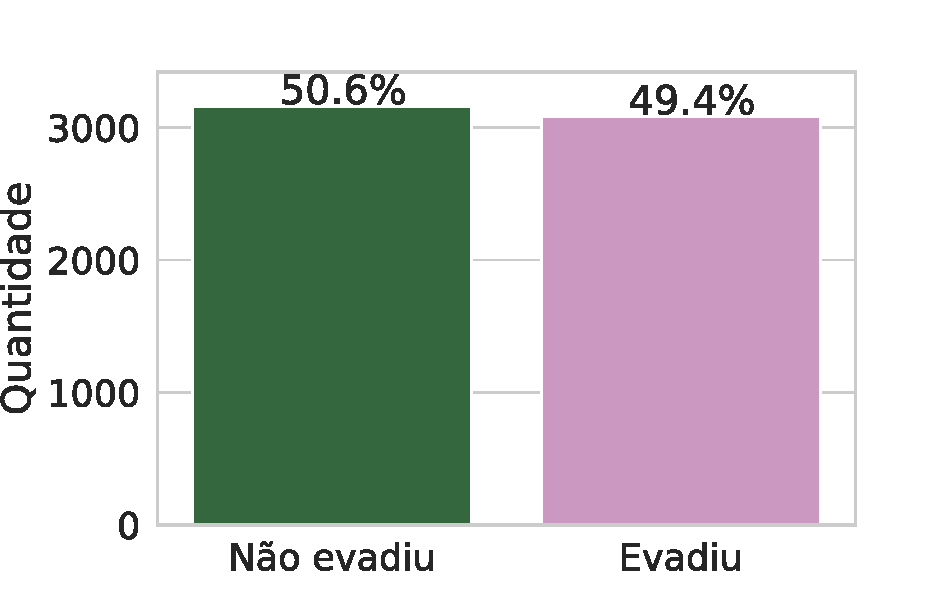
\includegraphics[scale=.29]{img/barplot_pedagogia}}\qquad
  \subcaptionbox{\label{classDistribuitionPedTest}Distribuição para os dados de teste.}{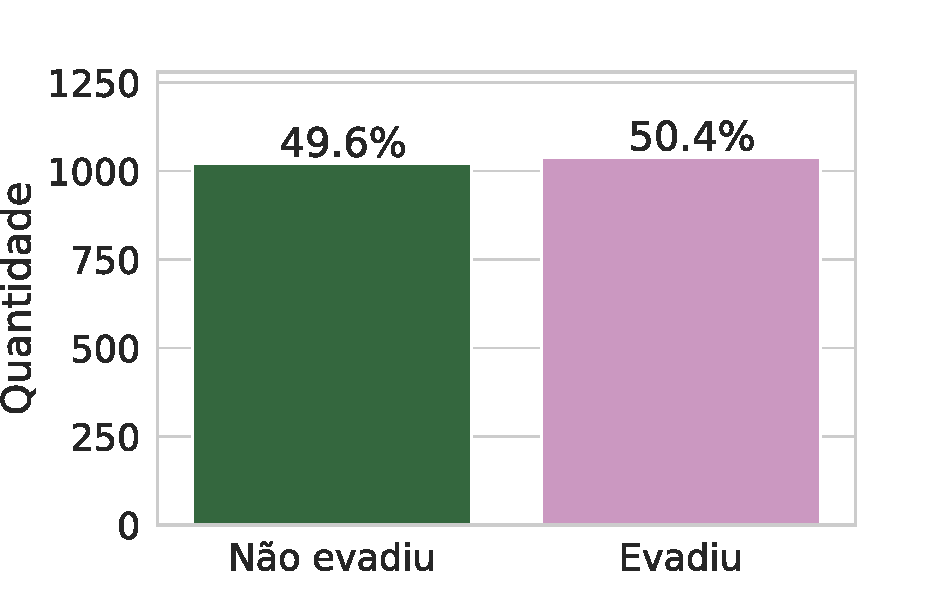
\includegraphics[scale=.29]{img/barplot_pedagogia_testes}}\qquad
  \subcaptionbox{\label{classDistribuitionPedTrain}Distribuição para os dados de treinamento.}{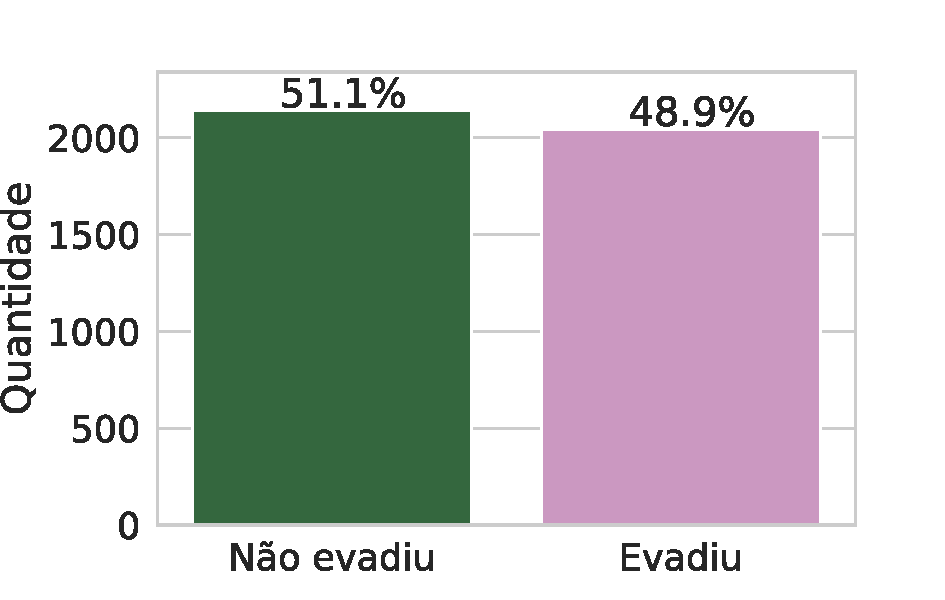
\includegraphics[scale=.29]{img/barplot_pedagogia_treinamento}}
  \vspace{1.5em}
  \Ididthis
\end{figure}

Os dados do curso de Bacharelado em Administração Pública somaram 11685
entradas. Sendo que, $43,9\%$ foram marcados como não evadidos e $56,1\%$ foram
marcados como evadido, como ilustra a Figura \ref{classDistribuitionAdmTotal}. A
proporção das classes após a divisão dos dados em conjunto de testes e conjunto
de treinamento é mostrada nas Figuras \ref{classDistribuitionAdmTest} e
\ref{classDistribuitionAdmTrain}, respectivamente.

\begin{figure}[!htb]
  \centering
  \caption{\label{classDistribuitionAdm} Distribuição de classes para os dados do curso de Bacharelado em Administração Pública.}
  \subcaptionbox{\label{classDistribuitionAdmTotal}Distribuição em todos os dados.}{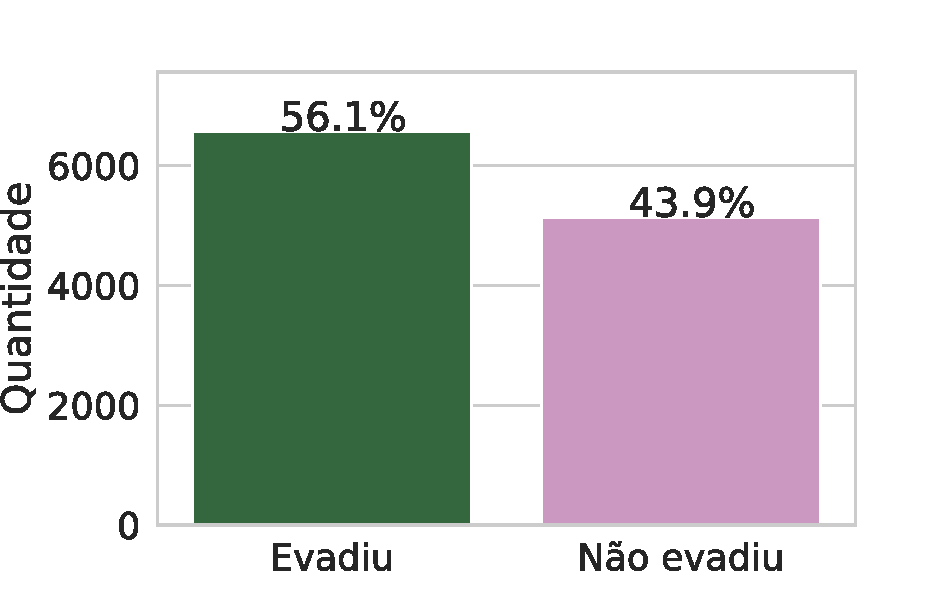
\includegraphics[scale=.29]{img/barplot_adm}}\qquad
  \subcaptionbox{\label{classDistribuitionAdmTest}Distribuição para os dados de teste.}{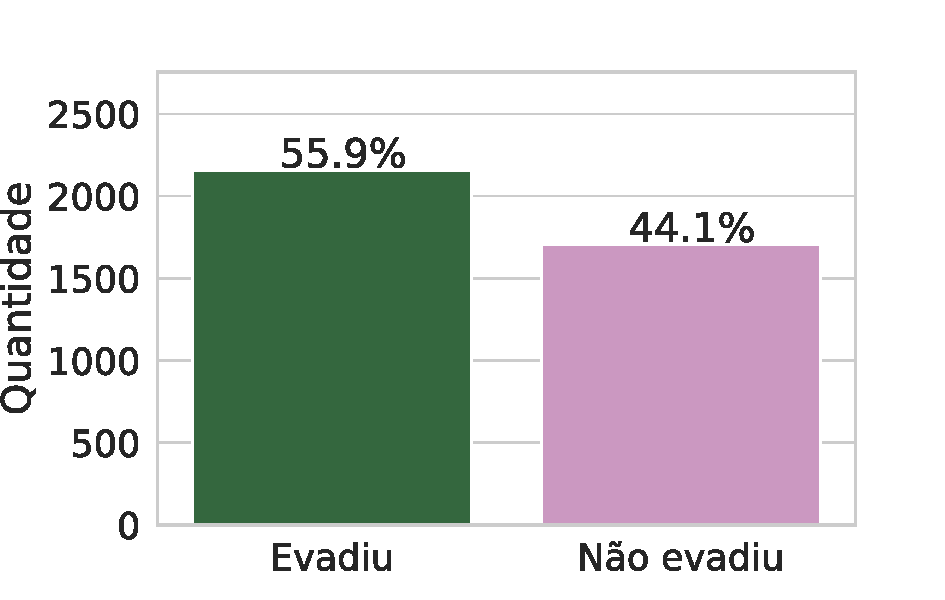
\includegraphics[scale=.29]{img/barplot_adm_testes}}\qquad
  \subcaptionbox{\label{classDistribuitionAdmTrain}Distribuição para os dados de treinamento.}{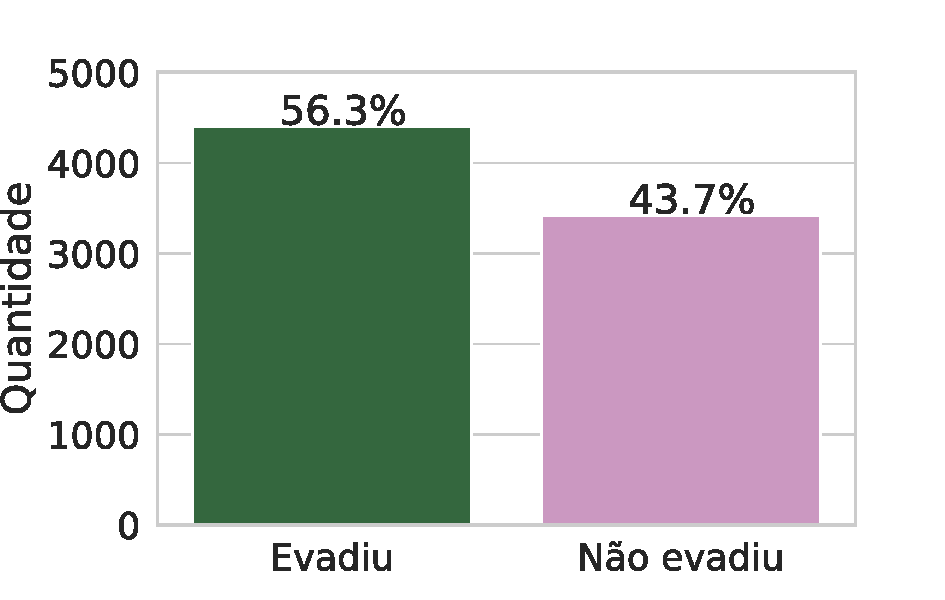
\includegraphics[scale=.29]{img/barplot_adm_treinamento}}
  \vspace{1.5em}
  \Ididthis
\end{figure}

Já que os conjuntos de dados mantiveram proporções semelhantes, os conjuntos de
teste servirão como conjuntos de validação, as matrizes de confusão e as
métricas serão calculadas utilizando-os.

As Tabelas \ref{decribingStatisticsPed} e \ref{decribingStatisticsAdm}
apresentam as estatísticas descritivas das variáveis coletadas no curso de
Licenciatura em Pedagogia e Bacharelado em Administração Pública,
respectivamente.

\begin{table}[!htb]
  \centering
  \caption{Estatísticas descritivas para as variáveis do curso de Licenciatura em Pedagogia}
  \label{decribingStatisticsPed}
  \begin{tabular}{@{}lrrrr@{}}
    \toprule
    \multicolumn{1}{c}{\textbf{Variável}} & \multicolumn{1}{c}{\textbf{Min}} & \multicolumn{1}{c}{\textbf{Média}} & \multicolumn{1}{c}{\textbf{Mediana}} & \multicolumn{1}{c}{\textbf{Max}} \\ \midrule
    VAR01 & 0,00 & 2,19 & 0,00 & 49,00 \\
    VAR02 & 0,00 & 20,45 & 4,00 & 956,00 \\
    VAR03 & 0,00 & 43,46 & 28,00 & 356,00 \\
    VAR04 & 0,00 & 12,89 & 14,00 & 36,00 \\
    VAR05a & 0,00 & 15,91 & 7,00 & 157,00 \\
    VAR05b & 0,00 & 25,77 & 15,00 & 215,00 \\
    VAR05c & 0,00 & 36,70 & 19,00 & 314,00 \\
    VAR06 & 0,00 & 2,89 & 0,00 & 115,00 \\
    VAR07 & 0,00 & 80,87 & 57,00 & 604,00 \\
    VAR08 & 0,00 & 9,82 & 2,00 & 241,00 \\
    VAR09 & 0,00 & 30,39 & 21,00 & 194,00 \\
    VAR10 & 0,00 & 6,79 & 1,00 & 102,00 \\
    VAR11 & 0,00 & 6,78 & 0,00 & 539,00 \\
    VAR12 & 0,00 & 0,29 & 0,00 & 5,00 \\
    VAR12 & 0,00 & 3,97 & 2,67 & 117,17 \\
    VAR14 & 0,00 & 4,71 & 4,00 & 28,00 \\
    VAR15 & 0,00 & 17,74 & 3,00 & 684,00 \\ \bottomrule
  \end{tabular}
\end{table}

\begin{table}[!htb]
  \centering
  \caption{Estatísticas descritivas para as variáveis do curso de Bacharelado em Administração Pública}
  \label{decribingStatisticsAdm}
  \begin{tabular}{@{}lrrrr@{}}
    \toprule
    \textbf{Variável} & \multicolumn{1}{l}{\textbf{Min}} & \multicolumn{1}{l}{\textbf{Média}} & \multicolumn{1}{l}{\textbf{Mediana}} & \multicolumn{1}{l}{\textbf{Max}} \\ \midrule
    VAR01 & 0,00 & 1,42 & 0,00 & 59,00 \\
    VAR02 & 0,00 & 21,66 & 2,00 & 1797,00 \\
    VAR03 & 0,00 & 61,59 & 43,00 & 1114,00 \\
    VAR04 & 0,00 & 17,70 & 17,00 & 81,00 \\
    VAR05a & 0,00 & 20,60 & 7,00 & 402,00 \\
    VAR05b & 0,00 & 27,46 & 14,00 & 342,00 \\
    VAR05c & 0,00 & 29,96 & 15,00 & 272,00 \\
    VAR06 & 0,00 & 1,09 & 0,00 & 96,00 \\
    VAR07 & 0,00 & 80,40 & 50,00 & 1000,00 \\
    VAR08 & 0,00 & 13,22 & 1,00 & 346,00 \\
    VAR09 & 0,00 & 48,89 & 32,00 & 471,00 \\
    VAR10 & 0,00 & 5,22 & 0,00 & 626,00 \\
    VAR11 & 0,00 & 5,08 & 0,00 & 1598,00 \\
    VAR12 & 0,00 & 0,13 & 0,00 & 6,00 \\
    VAR12 & 0,00 & 2,65 & 1,67 & 55,10 \\
    VAR14 & 0,00 & 4,66 & 5,00 & 20,00 \\
    VAR15 & 0,00 & 9,55 & 0,00 & 533,00 \\ \bottomrule
  \end{tabular}
\end{table}

Sabendo-se dessas informações, principiaram-se os experimentos com os algoritmos
de classificação. Destes, o primeiro foi o KNN. Iniciou-se pela escolha do
parâmetro \(k\), a quantidade de vizinhos. Para tal, foram testados valores
entre \(3\) e \(201\), mantendo-se sempre uma quantidade impar de vizinhos. Esse
experimento foi repetido, porém, com os dados normalizados, na tentativa de
remover a influência da diferença de escalas entre as variáveis.

A acurácia do algoritmo foi escolhida como métrica nesses experimentos por ser
uma métrica clássica e utilizada como padrão na biblioteca \textit{Scikt-learn}.

A partir da análise dos gráficos gerados, foi escolhido o valor \(3\) para o
parâmetro \(k\) na aplicação do KNN sobre os dados do curso de Licenciatura em
Pedagogia e o valor \(1\) para o curso de Bacharelado em Administração Pública.

Os algoritmos Árvore de Decisão e Regressão Logística não possuem parâmetros,
portanto, não tiveram que passar pelo mesmo processo que o KNN.

Notou-se que a variável \textit{VAR07} (Quantidade de acessos do aluno ao
ambiente no semestre) apareceu como a mais relevante. Porém, como todas as
outras variáveis só são contabilizadas depois que o aluno acessa o ambiente,
essa variável se torna bastante enviesada. Devido a isso, a etapa de mineração
foi executada novamente com a exclusão da mesma.

Para o algoritmo KNN, o valor de \(k\) foi ajustado para os dados sem a variável
\textit{VAR07}. As Figuras \ref{knnKResultsPedNoVar7} e
\ref{knnResultsAdmNoVar7} ilustram os gráficos utilizados para a escolha do
parâmetro \(k\).

\begin{figure}[!htb]
  \centering
  \caption{\label{knnKResultsPedNoVar7} Gráficos de valores de acurácia para valores de K, com K variando entre \(3\) e \(201\) com incremento de \(2\) para o curso de Licenciatura em Pedagogia após a exclusão da variável \textit{VAR07}.}
  \subcaptionbox{\label{knnKResultsPedANoVar7A}Dados não normalizados.}{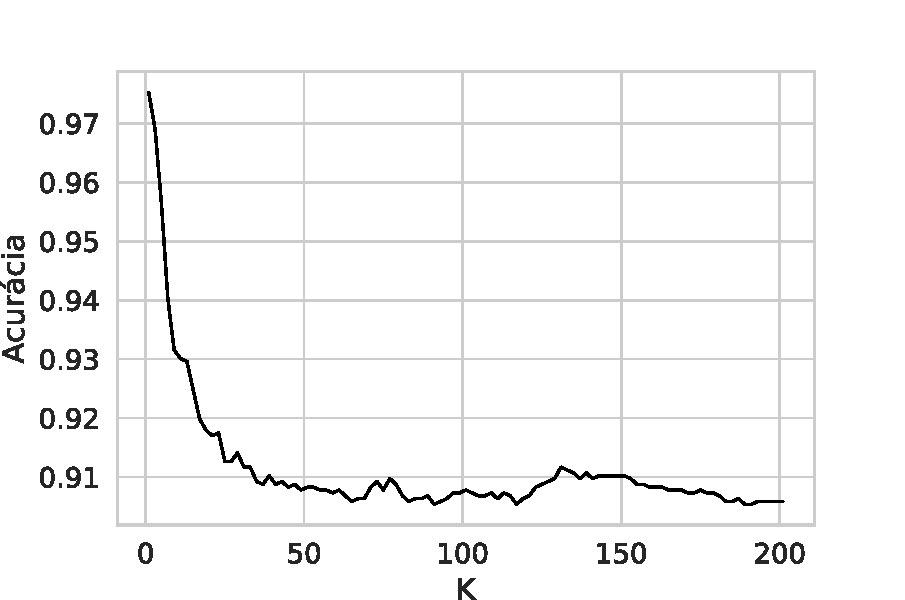
\includegraphics[scale=.45]{img/knn_neigh_ped_no_var07}}\qquad
  \subcaptionbox{Dados normalizados.}{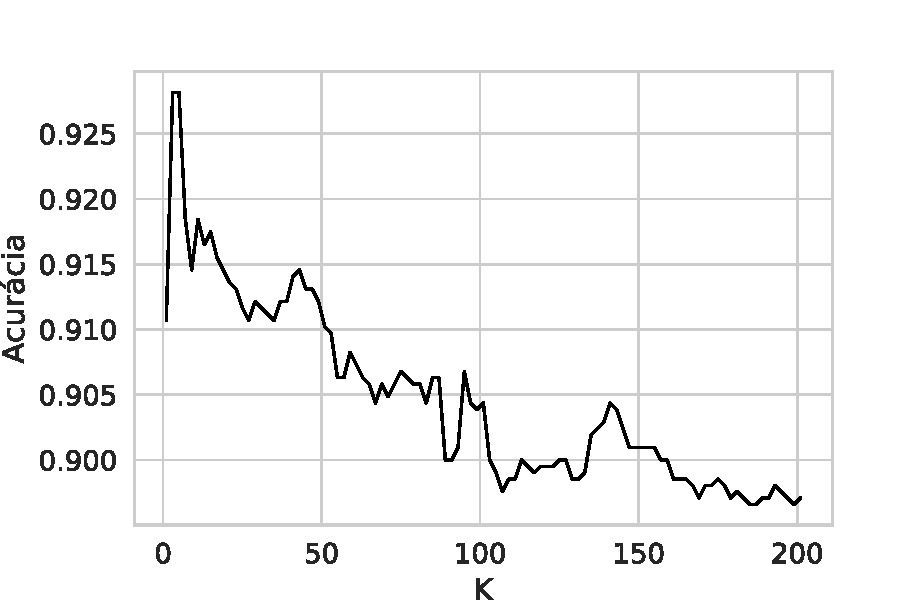
\includegraphics[scale=.45]{img/knn_neigh_norm_ped_no_var07}}
  \vspace{1.5em}
  \Ididthis
\end{figure}

\begin{figure}[!htb]
  \centering
  \caption{\label{knnResultsAdmNoVar7} Gráficos de valores de acurácia para valores de K, com K variando entre \(3\) e \(201\) com incremento de \(2\) para o cuso de Bacharelado em Administração Pública após a exclusão da variável \textit{VAR07}.}
  \subcaptionbox{\label{knnKResultsAdmANoVar7A}Dados não normalizados.}{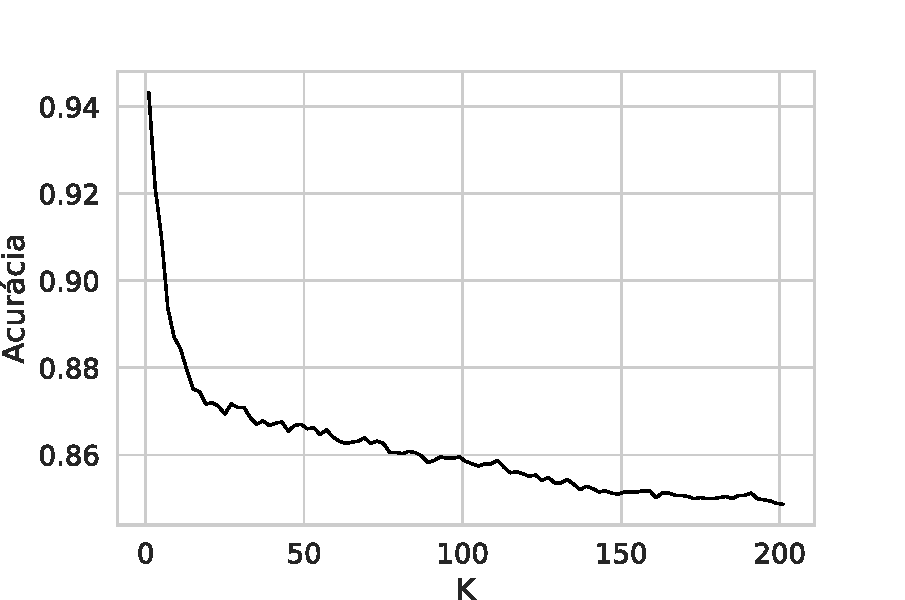
\includegraphics[scale=.45]{img/knn_neigh_adm_no_var07}}\qquad
  \subcaptionbox{Dados normalizados.}{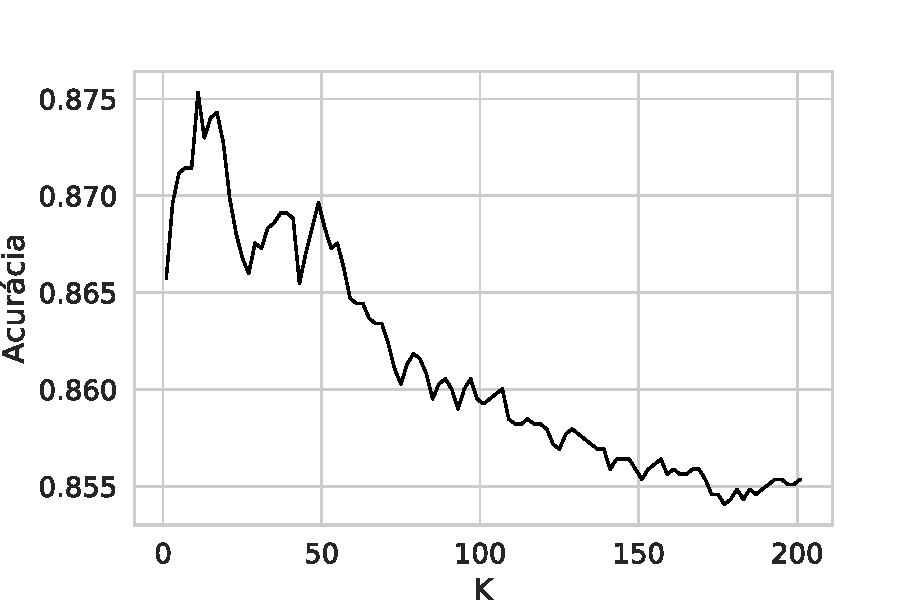
\includegraphics[scale=.45]{img/knn_neigh_norm_adm_no_var07}}
  \vspace{1.5em}
  \Ididthis
\end{figure}

Após análise dos gráficos contidos nas Figuras \ref{knnKResultsPedANoVar7A} e
\ref{knnKResultsAdmANoVar7A}, optou-se para valores de \(k = 1\) e os dados não
normalizados em ambas as bases.

Em seguida, foram geradas novas matrizes de confusão que estão ilustradas na Figura \ref{newConfusionMatrixResult}.

As matrizes de confusão serviram como base para o cálculo das métricas dos
algoritmos de classificação, as Tabelas \ref{metricsPed} e \ref{metricsAdm}
apresentam os resultados para cada algoritmo.

\begin{figure}[!htb]
  \centering
  \caption{\label{newConfusionMatrixResult} Matrizes de confusão após a exclusão da \textit{VAR07}.}
  \subcaptionbox{KNN Administração.}{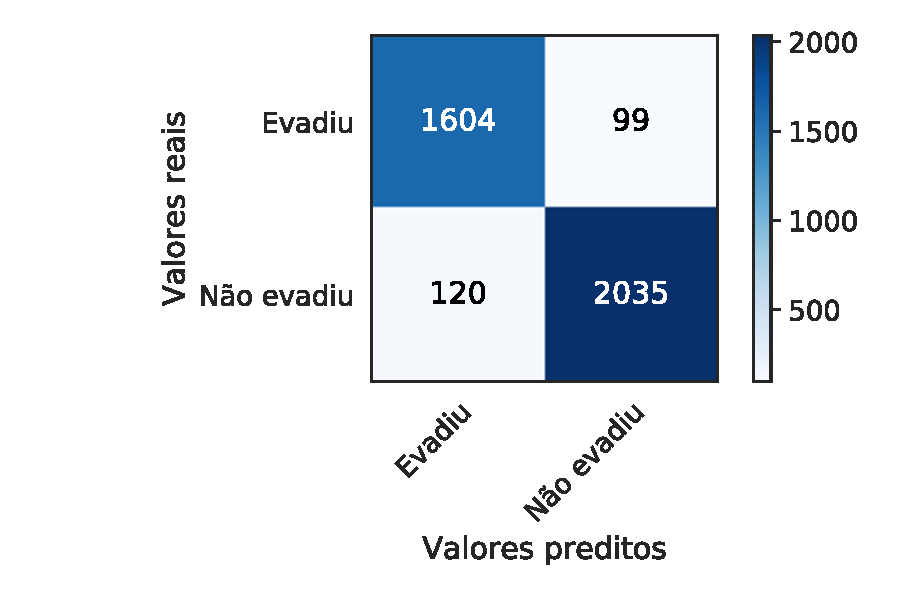
\includegraphics[scale=.40]{img/cm_knn_adm_no_var07}}\qquad
  \subcaptionbox{LR Administração.}{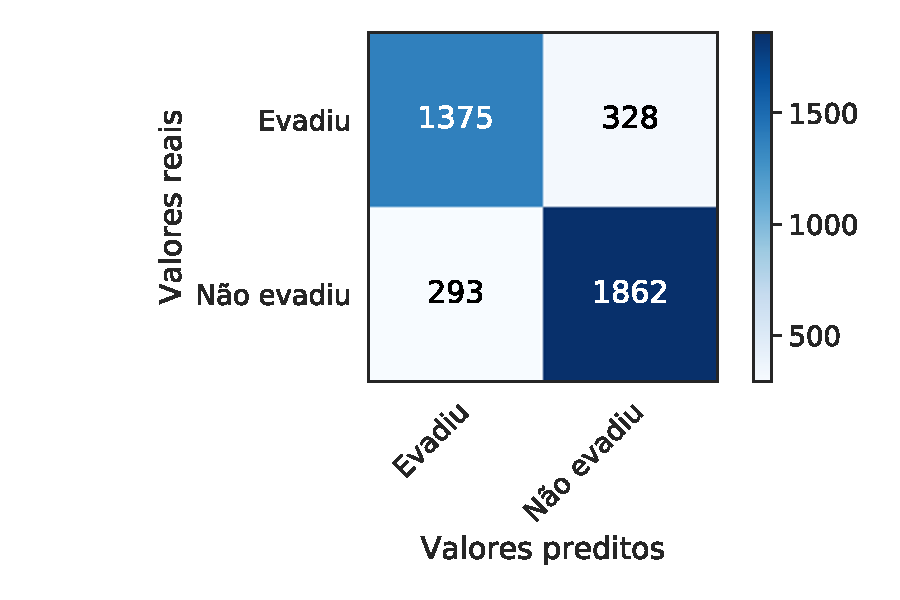
\includegraphics[scale=.40]{img/cm_rl_adm_no_var07}}\qquad
  \subcaptionbox{Árvore de Decisçao Administração.}{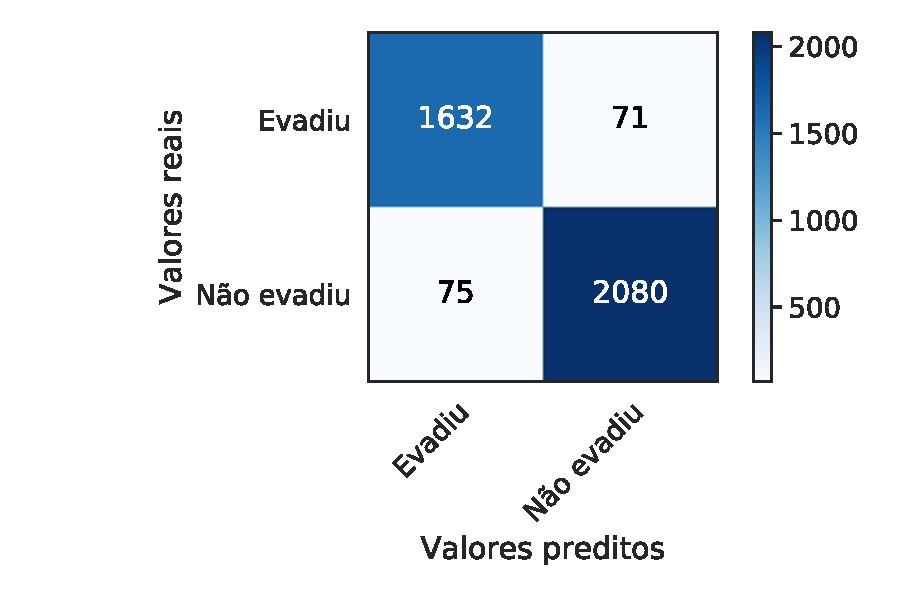
\includegraphics[scale=.40]{img/cm_tree_adm_no_var07}}
  \subcaptionbox{KNN Pedagogia.}{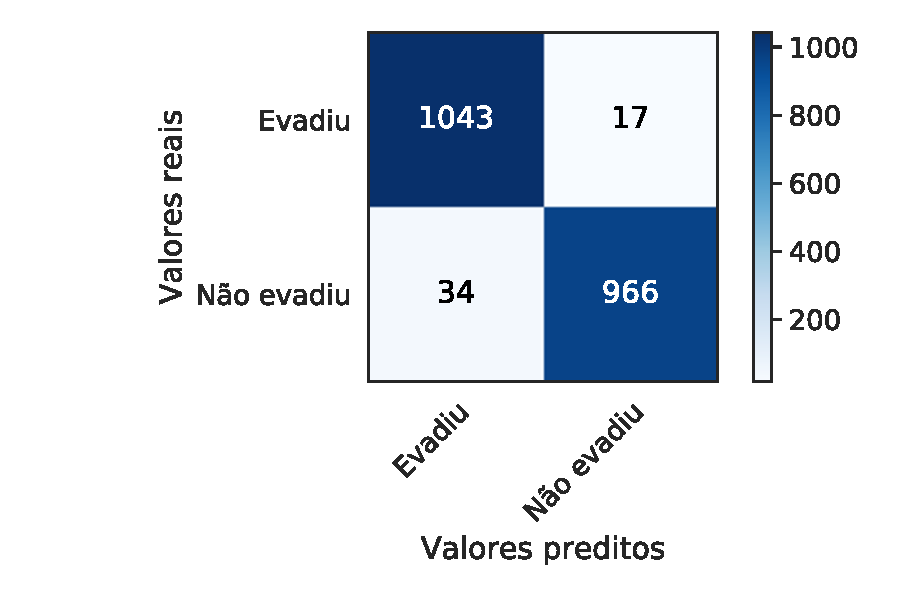
\includegraphics[scale=.40]{img/cm_knn_ped_no_var07}}\qquad
  \subcaptionbox{LR Pedagogia.}{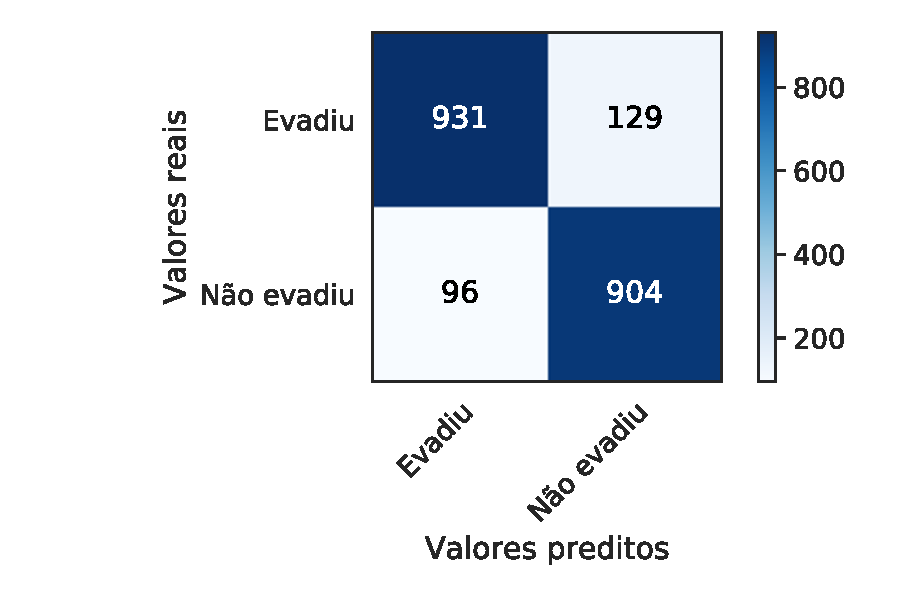
\includegraphics[scale=.40]{img/cm_rl_ped_no_var07}}\qquad
  \subcaptionbox{Árvore de Decisçao Pedagogia.}{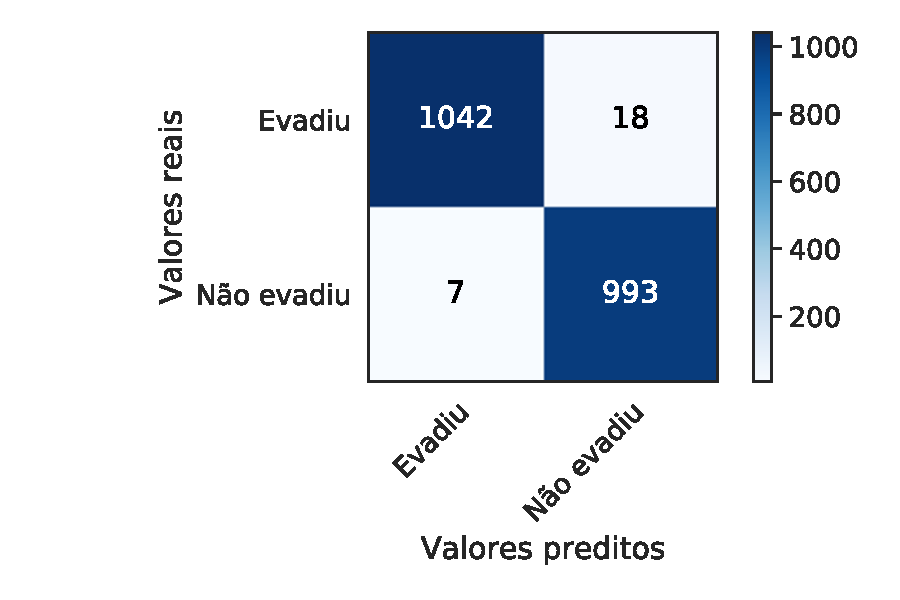
\includegraphics[scale=.40]{img/cm_tree_ped_no_var07}}
  \vspace{1.5em}
  \Ididthis
\end{figure}

Também foi realizada a análise da árvore de decisão gerada depois da remoção da
variável \textit{VAR07}. A representação gráfica das árvores para o curso de
Licenciatura em Pedagogia e Bacharelado em Administração Pública estão
ilustradas nas Figuras \ref{treePedNoVar07} e \ref{treeAdmNoVar07},
respectivamente.

\begin{figure}[!htb]
  \centering
  \caption{\label{treePedNoVar07} Árvore de Decisão gerada a partir dos dados do curso de Licenciatura em Pedagogia.}
  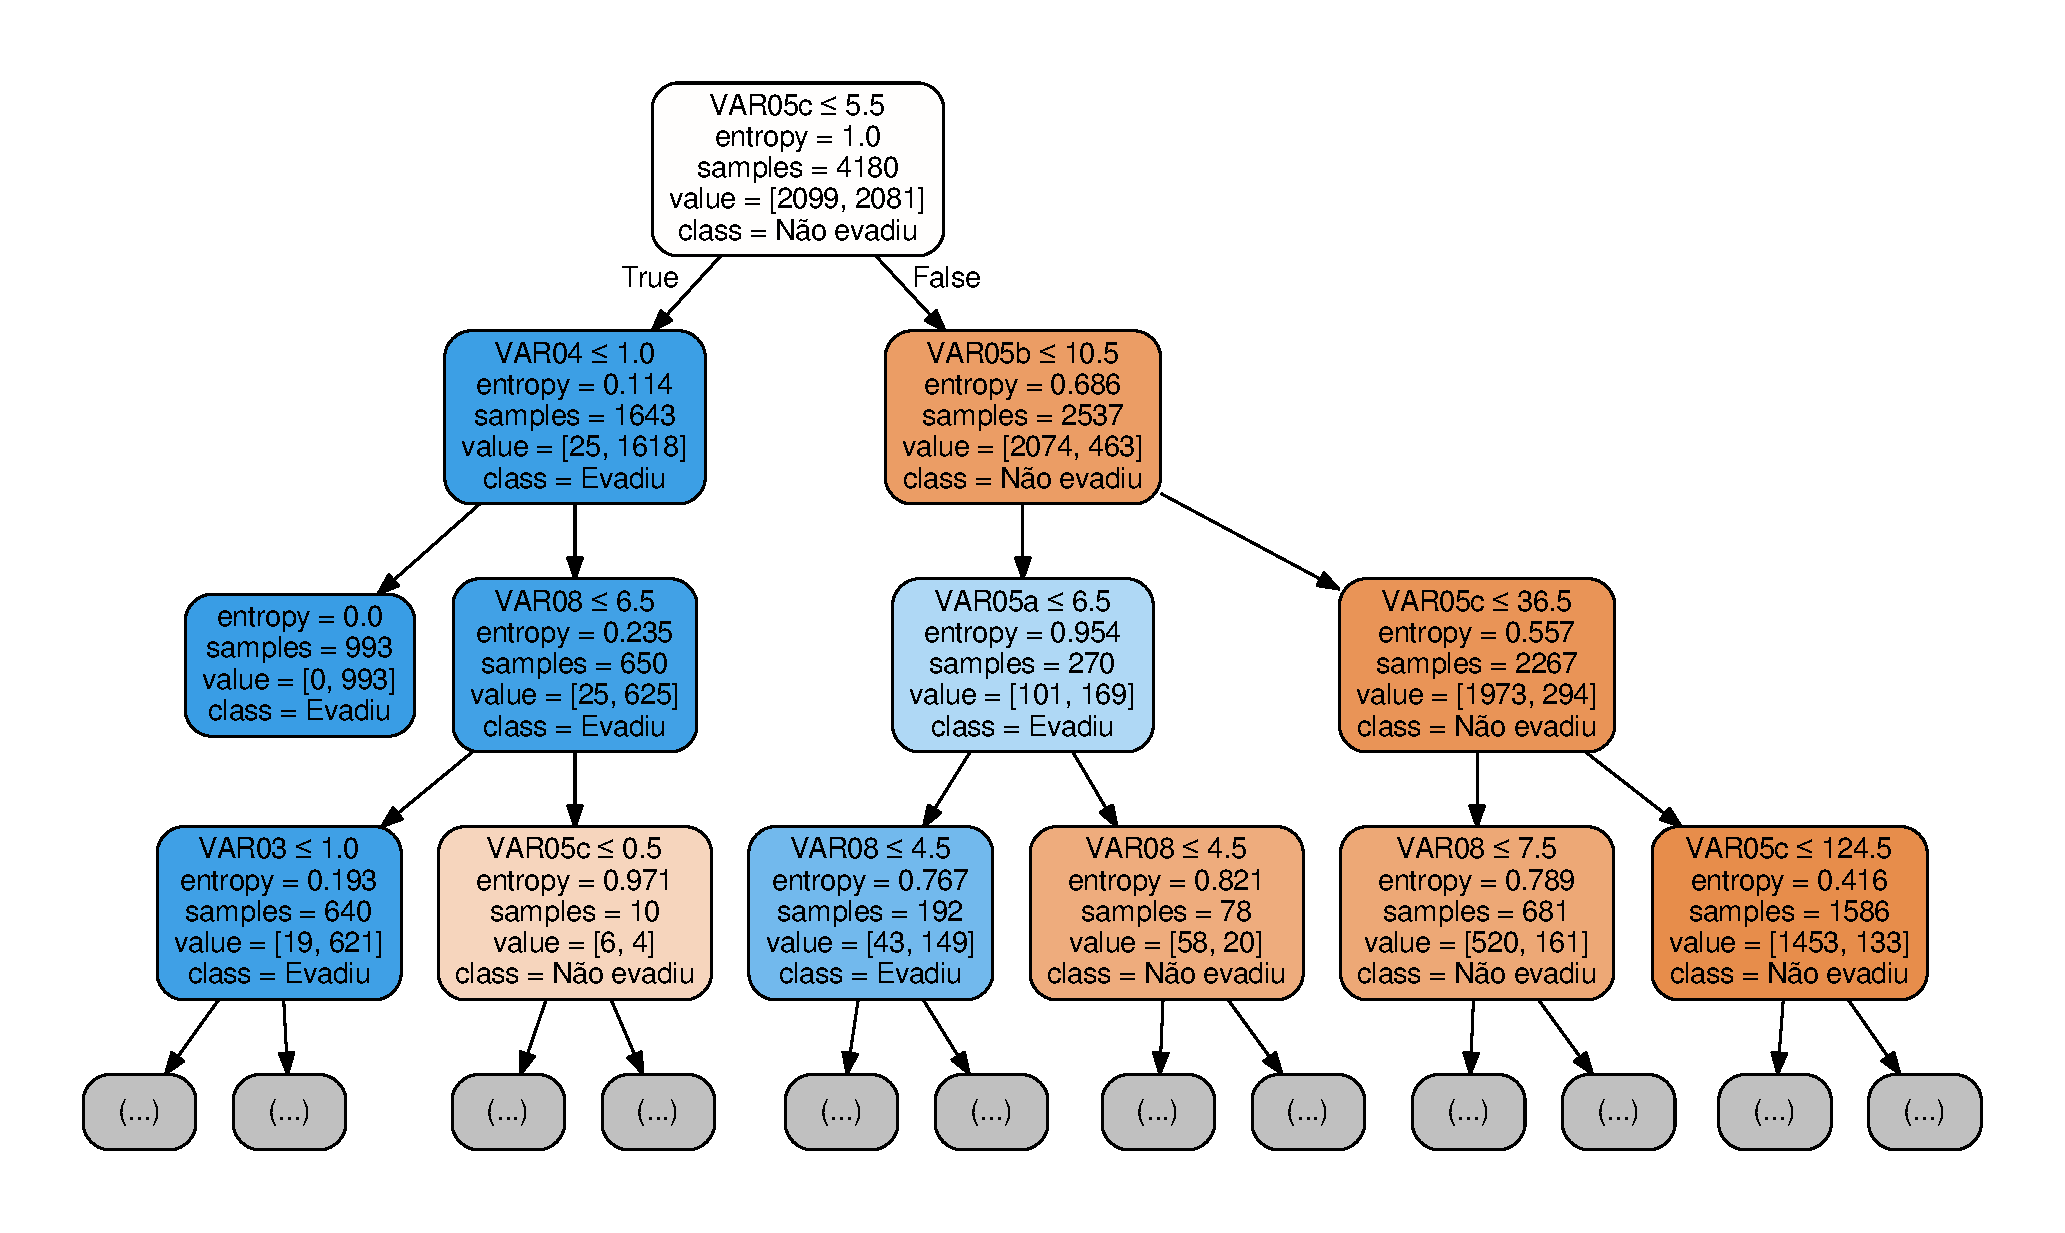
\includegraphics[angle=-90,scale=.50]{img/ped_tree_no_var07}
  \Ididthis
\end{figure}

\begin{figure}[!htb]
  \centering
  \caption{\label{treeAdmNoVar07} Árvore de Decisão gerada a partir dos dados do curso de Bacharelado em Administração Pública.}
  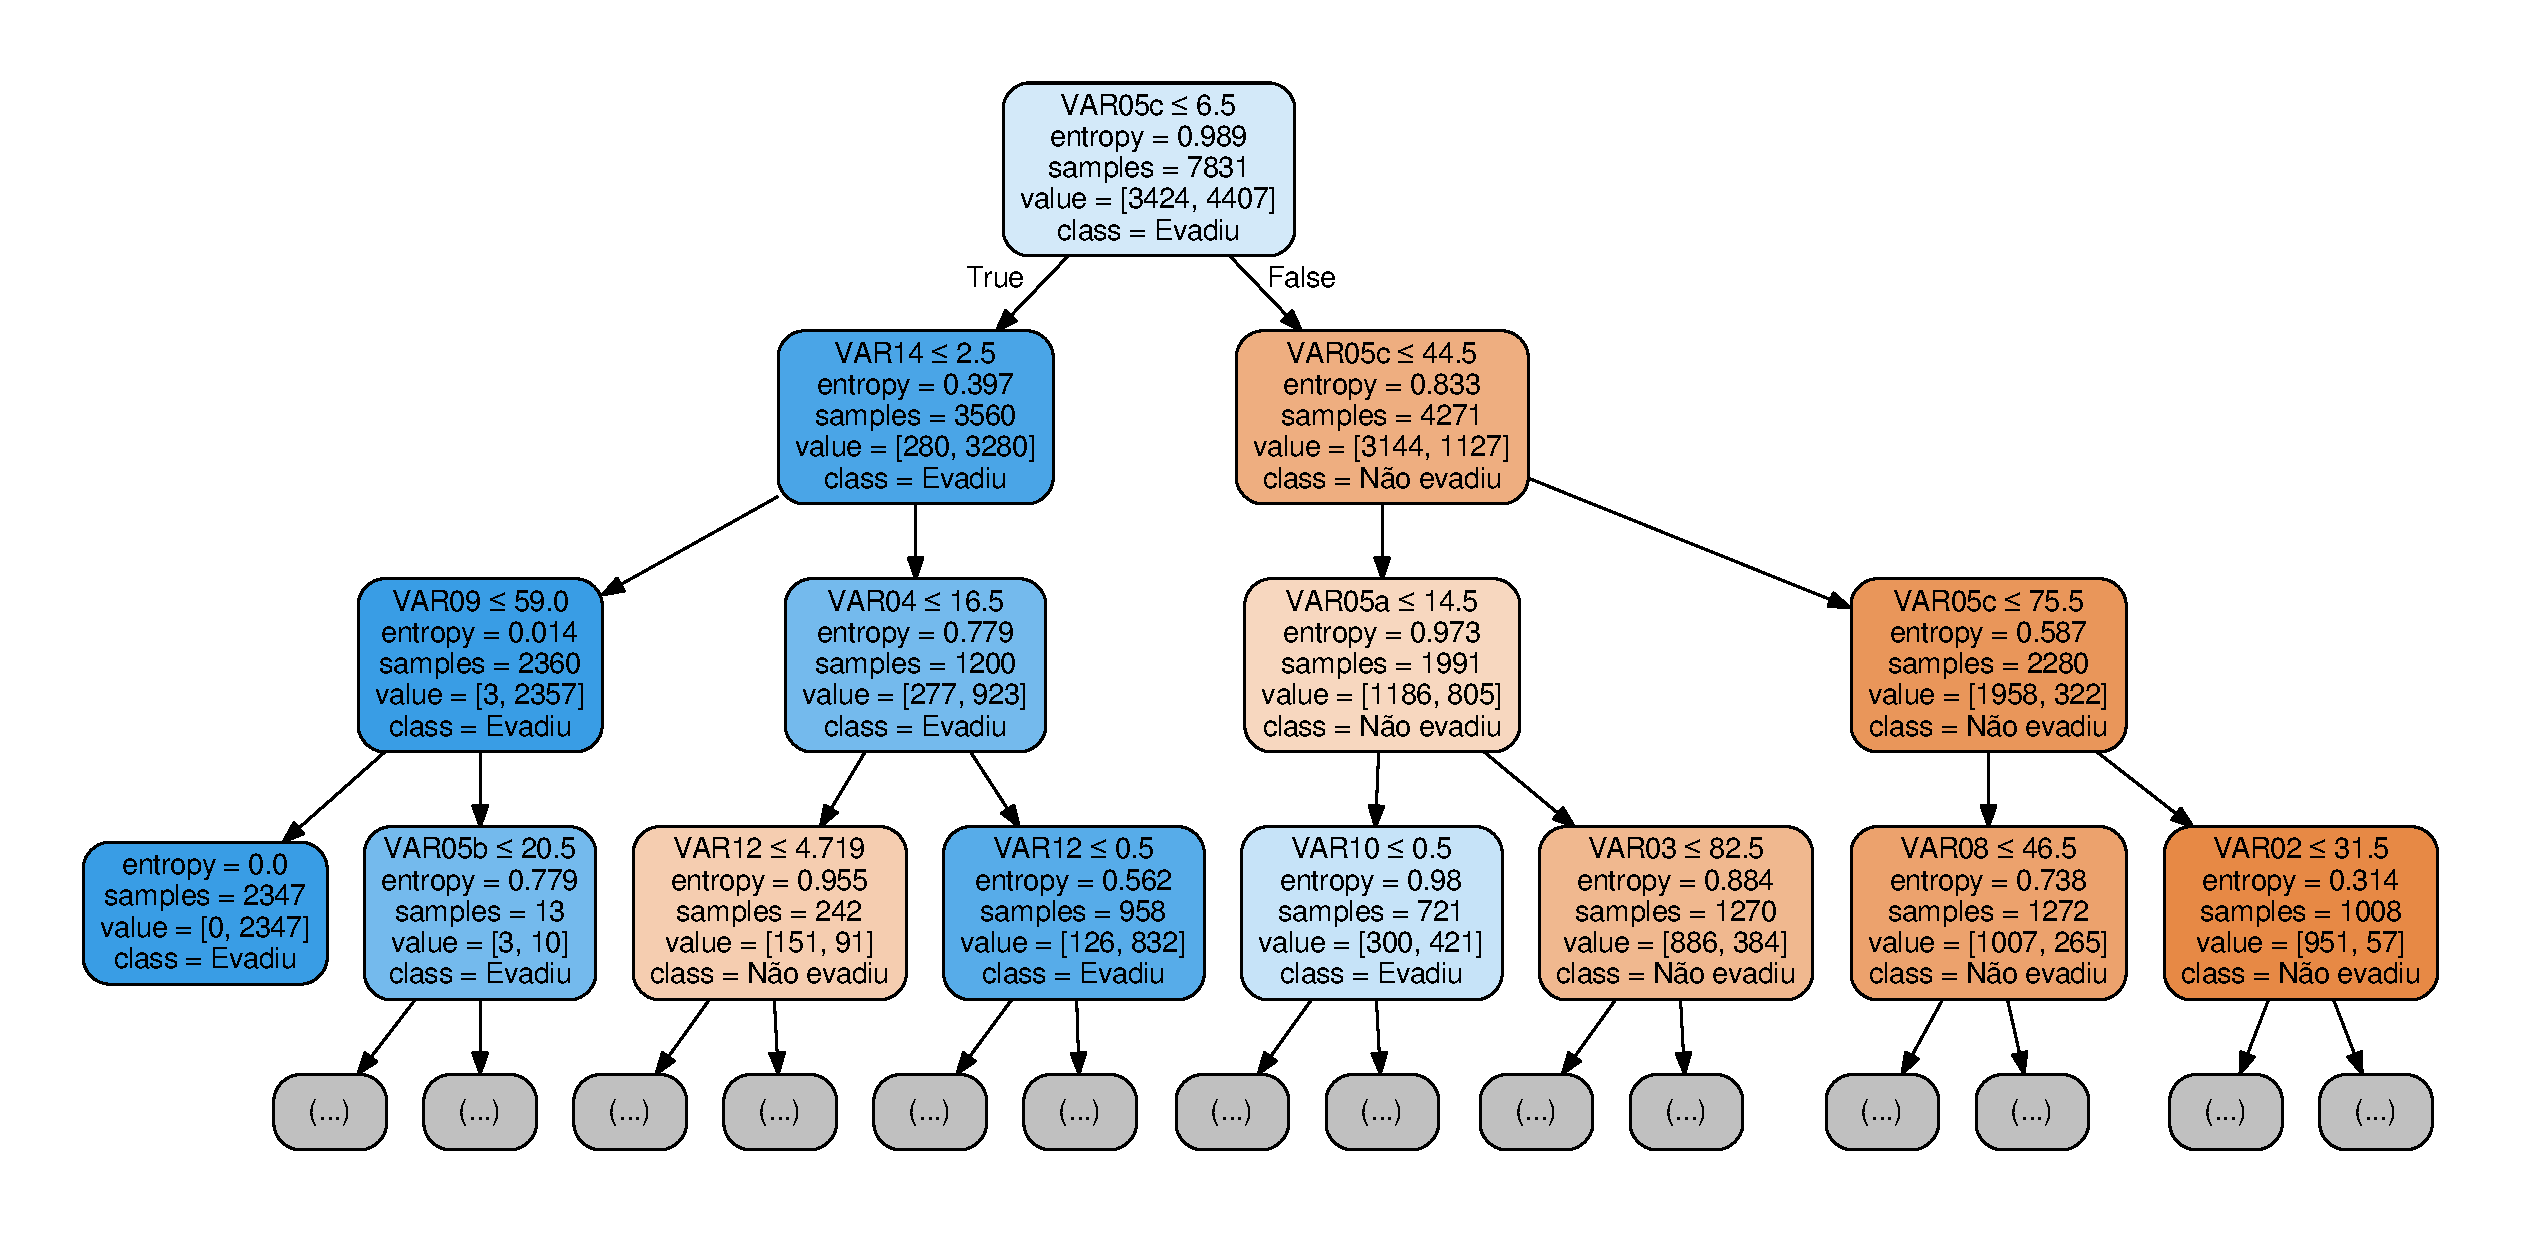
\includegraphics[angle=-90,scale=.50]{img/adm_tree_no_var07}
  \Ididthis
\end{figure}

Nas novas árvores, a variável com maior importância foi a \textit{VAR05c}, que
representa a quantidade de acessos do aluno ao ambiente no período da noite, por
semestre.

\section{Pós-processamento}

Os dados foram convertidos para formato CSV de forma que podem ser utilizados no
futuro para treinamento ou validação de outros algoritmos de classificação.

Os  scripts e visualizações geradas foram disponibilizadas publicamente em um
repositório público.

\section{Conhecimentos Obtidos}

A análise dos dados permitiu perceber que os alunos da EAD na UNIVASF tendem a
evadir entre o quarto e quinto semestre do curso.

Os algoritmos de classificação apresentaram métricas compatíveis com as
encontradas na literatura.

Para o curso de Licenciatura em Pedagogia, o algoritmo Árvore de Decisão foi o
que obteve as melhores métricas, com exceção da sensibilidade, onde ele ficou
abaixo do KNN. A variável com maior importância, segundo o gráfico da árvore,
foi a \textit{VAR07} seguida pelas \textit{VAR04}, \textit{VAR08} e
\textit{VAR14}.

O mesmo comportamento foi observado para o curso de Bacharelado em Administração
Pública. O fato da variável \textit{VAR07} (Quantidade de acessos do aluno ao
ambiente no semestre --- Autonomia), ter sido destacada como mais importante em
ambos os cursos é explicado pelo fato da mesma a variável que define a principal
característica de um aluno evadir-se ou não, afinal sem acessar o ambiente
virtual, nenhum recurso pode ser visualizado e nenhuma atividade pode ser
executada, nenhum comportamento do aluno pode ser verificado, além do baixo ou
nenhum acesso aos cursos. Além disso, o fato da mesma apresentar uma grande
variabilidade em seus valores, pode também ter influenciado nessa importância em
relação às demais.

Após a segunda análise, sem a variável \textit{VAR007}, a que obteve maior
importância, para a árvore de decisão, foi a \textit{VAR05c}, apesar de ainda
ser uma variável relativa a quantidade de acessos, ela revela que os alunos que
acessam o ambiente durante a noite são os que possuem menores chances de evasão.

\section{Considerações Finais do Capítulo}

Neste capítulo foram apresentados os resultados obtidos em cada etapa do KDD
aplicada neste trabalho, foi verificado a distribuição das classes nos conjuntos
de dados, as estatísticas descritivas das variáveis, as métricas dos algoritmos
de classificação e as visualizações das árvores de decisão.

No proximo capítulo, serão apresentadas as considerações finais desta pesquisa e
sugestões de trabalhos futuros.

		\chapter{Considerações Finais e Trabalhos Futuros}

A modalidade EAD ajuda a democratizar o ensino, levando-o às regiões de difícil
acesso aos professores ou dando a oportunidade ao estudante de criar sua própria
rotina de estudos. A evasão desta modalidade de ensino ainda é um grande
problema a ser resolvido, logo, existe a necessidade de pesquisa científica
nesta área.

Com o uso crescente de ferramentas de tecnologia da informação em EAD fica
evidente que o uso de aprendizagem de máquina pode ser utilizado para modelar e
prever os fenômenos que causam a evasão.

O fluxo de descoberta de conhecimento em bases de dados descrito na metodologia
deste trabalho foi utilizado como arcabouço para a aplicação dos algoritmos de
classificação que foram comparados segundo métricas consolidadas na literatura.
Os resultados obtidos foram satisfatórios, aproximando-se aos encontrados na
literatura.

Os resultados obtidos neste trabalho, apontam que o uso das variáveis obtidas 
a partir dos contrutos da Teoria da Distância Transacional, podem ser usadas 
em ferramentas ou modelos preditivos da evasão dos alunos na EAD na UNIVASF, 
contemplando o objetivo geral do projeto.

Como trabalhos futuros, propõe-se a elaboração de um sistema de controle para
professores e gestores, que, integrado a um modelo de classificação, ajude a executar
alguma ação no curso antes que a evasão do aluno ocorra. Sinalizações automáticas de 
alunos com risco de evasão podem ser implementadas, para alertar professores e tutores 
sobre essa situação.
Além disso, um estudo aprofundado sobre relevância das variáveis preditoras, pode levar 
a uma redução da dimensionalidade das variáveis, sem perda do poder preditivo dos modelos. 
Isso pode impactar na perfomance do processo, pois com menos variáveis, uma menor quantidade 
de consultas ao banco de dados e um menor tempo de processamento dos modelos podem ser alcançados.


	\postextual
		\bibliography{tex/references}
		\begin{anexosenv}
  \chapter{Scripts SQL Utilizados Nesse Trabalho} \label{anex:anexo1}

  \sourcecodenolist{Script para calcular data de inicio}{sql}{calculate_start_date.sql}

  \sourcecodenolist{Script para calcular data de fim}{sql}{calculate_end_date.sql}

  \sourcecodenolist{Script para remover espaços em branco internos}{sql}{remove_inner_spaces.sql}

  \sourcecodenolist{Script para tratar os nomes dos semestres}{sql}{handle_semester.sql}

  \sourcecodenolist{Script para calcular o período}{sql}{calculate_period.sql}

  \sourcecodenolist{Script para remover espaços duplos}{sql}{remove_double_spaces.sql}

  \sourcecodenolist{Script para remover pontos}{sql}{remove_dots.sql}

  \sourcecodenolist{Script para criar as tabelas auxiliates}{sql}{create_base.sql}

  \sourcecodenolist{Script para criar a tabela de alunos}{sql}{create_view_alunos.sql}

  \sourcecodenolist{Script para criar a tabela de professores}{sql}{create_view_professores.sql}
\end{anexosenv}
\end{document}
